%====================================================
%	CHAPTER 4 - Control
%====================================================
\chapter{Controller Development}
\label{ch:control}
%====================================================
\section{Control Loop}
\label{sec:control.loop}
%====================================================
The control problem is, as outlined in Ch:\ref{ch:intro}, to achieve non-zero setpoint tracking (for both \emph{attitude} and \emph{position} states) on a quadrotor by solving the problem of its inherent underactuation. For the purposes of the subsequent controller development, the plant for some state $\vec{\mathbf{x}}$ is described in the following typical nonlinear state-space form in the time domain:
\begin{subequations}\label{eq:control-loop-states}
\begin{equation}
\frac{d}{dt}{\vec{\mathbf{x}}}=f(\vec{\mathbf{x}},t)+g(\vec{\mathbf{x}},\vec{\nu},t)
\end{equation}
\vspace{-12pt}
\begin{equation}
\vec{y} = c(\vec{\mathbf{x}},t)+d(\vec{\mathbf{x}},\vec{\nu},t)
\end{equation}
\end{subequations}
where the plant's dynamics are governed by state progression $f(\vec{\mathbf{x}},t)$ and the plant's input response $g(\vec{\mathbf{x}},\vec{\nu},t)$ for a given control input $\vec{\nu}$. The latter could take the affine form $g(\vec{\mathbf{x}},t)\vec{\nu}$. Setpoint tracking aims for the output to track the plant's state; namely $\vec{y} = c(\vec{\mathbf{x}},t)\equiv\vec{\mathbf{x}}$. The control problem is then to design a stabilizing control law $\mathcal{H}$ for some error state difference between the desired and current state references, respectively $\vec{\mathbf{x}}_e=\vec{\mathbf{x}}_d-\vec{\mathbf{x}}_b$ and:
\begin{equation}
\vec{\nu}_d\triangleq\mathcal{H}(\vec{\mathbf{x}}_e,\dot{\vec{\mathbf{x}}}_e,t)=\mathcal{H}(\vec{\mathbf{x}}_b,\dot{\vec{\mathbf{x}}}_b,\vec{\mathbf{x}}_d,\dot{\vec{\mathbf{x}}}_d,t)=\begin{bmatrix}
\vec{F}_d &
\vec{\tau}_d
\end{bmatrix}^T
\end{equation}
such that the controlled plant's error is asymptotically stabilized, or that $\lim_{t\rightarrow\infty}\vec{\mathbf{x}}_e=\vec{0}$. Inputs $\vec{F}_d$ and $\vec{\tau}_d$ are controller designed force and torque inputs respectively, to be applied by the actuator set. Trajectory stability conditions are defined next in Sec:\ref{sec:control.stability}. Note that it is possible to combine attitude and position states into a single common trajectory reference such that its position is given by:
\\
\vspace{-5pt}
\begin{equation}
\vec{\mathbf{x}}_b=\begin{bmatrix}\vec{\mathcal{E}}_I&Q_b\end{bmatrix}^T
\end{equation}
The body's trajectory is then fully described by $\vec{\mathbf{x}}_b(t)$ and its derivative $\dot{\vec{\mathbf{x}}}_b(t)$. Separate control laws are developed for attitude and position tracking so both states are not combined in the context of this control project. Because the plant is overactuated, the control loop is split into two blocks; first a higher level \emph{setpoint tracking} controller designs a virtual control input $\vec{\nu}_d$, being net forces $\vec{F}_d$ and torques $\vec{\tau}_d$ to act on the body. Next, a lower level \emph{allocator} solves for explicit actuator positions using $\vec{\nu}_d$ to physically actuate that \emph{virtual} control input. The actuator a commands control input $\vec{\nu}_c(\vec{u}_c)$ through its effectiveness function, defined in Eq:\ref{eq:dynamic-plant-inputs}, where the commanded actuator positions $\vec{u}_c$ are subject to the transfer function $C(s)$ described in Sec:\ref{subsec:proto.design.transfer}.
\begin{equation}\label{eq:control-effectiveness}
\vec{\nu}_c=\begin{bmatrix}
\vec{F}_c(\vec{u}_c) & \vec{\tau}_c(\vec{u}_c)
\end{bmatrix}^T=B(\vec{\mathbf{x}},\vec{u}_c,t)
\end{equation}
where $\vec{F}_c(\vec{u}_c)$ and $\vec{\tau}_c(\vec{u}_c)$ are the respective commanded input forces and torques actuated by $\vec{u}_c$. 
\par
The allocator solves for commanded actuator values $\vec{u}_c$ such that $\vec{\nu}_c\rightarrow\vec{\nu}_d$. That allocation function, $B^\dagger$, can be \emph{roughly} referred to as the effectiveness inverse:
\begin{equation}
\vec{u}_c=B^{\dagger}(\vec{\mathbf{x}},\vec{\nu}_d,t)~~~~\in\mathbb{U}
\end{equation}
This chapter derives higher level controllers for $\vec{\nu}_d=\mathcal{H}(\vec{\mathbf{x}}_e,\dot{\vec{\mathbf{x}}}_e,t)$. Allocation rules are discussed next in Ch:\ref{ch:allocation}. A collection of attitude and position controllers is presented here and stability is proven with Lyapunov theory \cite{lyapunovconference}. Each controller is compared in the context of an overactuated quadrotor plant, similarly a series of allocation schemes are presented. Propagation delays of the actuator input $\vec{u}_c$ result from the actuator plant's transfer function $C(s)$. Those delays are assumed to have far slower time constants than the controller. If actuator estimates $\hat{u}_c$ (incorporating the transfer functions) are used for feedback compensation calculations then major loop controller coefficients will account for the minor loop errors between a commanded $\vec{u}_c$ and its estimate $\hat{u}_c$. Comparisons of the designed controllers as well as their explicit coefficients and efficacy are evaluated subsequently in Ch:\ref{ch:simulation}. 
\par
A generalized overactuated control loop consists of a series of cascaded control blocks (Fig:\ref{fig:control-loop}). From the trajectory's error state $\vec{\mathbf{x}}_e$, a control law designs a virtual control input $\vec{\nu}_d$ which is applied to the allocation block. The allocation law $B^{\dagger}(\vec{\mathbf{x}},\vec{\nu}_d,t)$ solves for physical actuator positions $u_c\in\mathbb{U}$. Commanded actuator (\emph{estimate}) positions affect a physical input $\vec{\nu}_c=B(\vec{\mathbf{x}},\hat{u},t)$, which is an input applied to the state's dynamics, Eq:\ref{eq:control-loop-states}. Finally the output tracking state is estimated with some filter paradigm $\hat{\mathbf{x}}=A(\vec{\mathbf{x}},t)$ which is fed back for error state calculation (Sec:\ref{sec:simulation.state}).
\begin{figure}[htbp]
\vspace{-6pt}
\centering
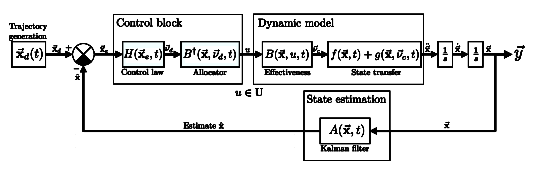
\includegraphics[width=0.9\textwidth]{figs/control-loop}
\vspace{-10pt}
\caption{Generalized control loop with allocation}
\vspace{-20pt}
\label{fig:control-loop}
\end{figure}
\par
Fig:\ref{fig:control-loop} shows a generalized overactuated control loop's structure which omits many of the intricacies associated with the model in question. Some aspects of the linear system of equations for the state transfer include multibody nonlinearities, derived in Sec:\ref{sec:dynamics.nonlinearities}, which are dependent on actuator positions and rates. That generalized case is now refined in the context of an overactuated quadcopter.
%====================================================
\section{Control Plant Inputs}
\label{sec:control.inputs}
%====================================================
Control inputs for the state's differential equations, from Eq:\ref{eq:quaternion-states}, have mostly been described with net input forces and torques; $\vec{F}_\mu(\hat{u})$ and $\vec{\tau}_\mu(\hat{u})$ respectively. The relationship of the \emph{effectiveness function} between each propeller's rotational speed and servo positions with the produced thrust vector is calculated from Eq:\ref{eq:quaternion-inputs}. For some (estimated) commanded actuator position $\hat{u}_c$:
\begin{subequations}\label{eq:control-input}
\begin{equation}
\vec{\nu}_c\triangleq\begin{bmatrix}
\vec{F}_c(\hat{u}_c) & \vec{\tau}_c(\hat{u}_c)
\end{bmatrix}^T=B(\vec{\mathbf{x}},\hat{u}_c,t)~~~~\in\mathbb{R}^6,~u_c\in\mathbb{U}
\end{equation}
\vspace{-12pt}
\begin{equation}
\vec{F}_\mu(\hat{u}_c)=\sum_{i=1}^4 Q_{M_i}^*(\lambda_i,\alpha_i)\otimes \vec{T}(\Omega_i)\otimes Q_{M_i}(\lambda_i,\alpha_i)~~~~\in\mathcal{F}^b
\end{equation}
\vspace{-6pt}
\begin{equation}
\vec{\tau}_\mu(\hat{u}_c)=\sum_{i=1}^4 \vec{L}_i\times\big(Q_{M_i}^*(\lambda_i,\alpha_i)\otimes \vec{T}(\Omega_i)\otimes Q_{M_i}(\lambda_i,\alpha_i)\big)~~~~\in\mathcal{F}^b
\end{equation}
\end{subequations}
As mentioned previously, a higher level controller $\mathcal{H}(\vec{\mathbf{x}}_e,\dot{\vec{\mathbf{x}}}_e,t)$ designs desired net plant inputs $\vec{\nu}_d=\begin{bmatrix}\vec{F}_d&\vec{\tau}_d\end{bmatrix}^T$ whilst a lower level allocator commands actuator positions $u_c=B^{\dagger}(\vec{\mathbf{x}},\vec{\nu}_d,t)$ such that $\vec{\nu}_c\rightarrow\vec{\nu}_d$. Actuator dynamics produce a tracking commanded input and not an instantaneously assumed actuator state. Separating the higher lever controller and lower level allocator accommodates comparison between the proposed controllers and respective allocation laws. However, typical allocation rules like pseudo-inversion require an invertible relationship between plant and control inputs, detailed previously in Sec:\ref{subsubsec:intro.lit.control.allocation} and expanded on next in Sec\ref{sec:allocation.slack}.
\par
The vector relationship in Eq:\ref{eq:control-input} is not reducible to a single multiplicative relationship between the commanded actuator matrix $\vec{u}_c\in\mathbb{U}\in\mathbb{R}^12$ (estimated or otherwise) and the dynamic plant input $\vec{\nu}_c\in\mathbb{R}^{6}$. So the effectiveness function needs an extra layer of abstraction to incorporate a multiplicative relationship. Rather than calculating explicit actuator positions directly from $\vec{\nu}_d$, a set of four 3-D thrust vectors $\vec{T}_{[1:4]}\in\mathbb{R}^{1\times 12}$ for each motor module is first calculated.
\begin{subequations}\label{eq:4.7}
\begin{equation}
\vec{\nu}_c=\begin{bmatrix}
\vec{F}_c(\hat{u}_c)\\
\vec{\tau}_c(\hat{u}_c)
\end{bmatrix}
= 
\begin{bmatrix}
\mathbb{I}_{3\times 3} & \mathbb{I}_{3\times 3} & \mathbb{I}_{3\times 3} & \mathbb{I}_{3\times 3}\\
[\vec{L}_1]_\times & [\vec{L}_2]_\times & [\vec{L}_3]_\times & [\vec{L}_4]_\times
\end{bmatrix}
\begin{bmatrix}
\vec{T}_1&
\vec{T}_2&
\vec{T}_3&
\vec{T}_4
\end{bmatrix}^T
\end{equation}
\vspace{-10pt}
\begin{equation}
\therefore\vec{\nu}_c=B'(\vec{\mathbf{x}},t)\begin{bmatrix}
\vec{T}_1&
\vec{T}_2&
\vec{T}_3&
\vec{T}_4
\end{bmatrix}^T
\end{equation}
\vspace{-10pt}
\begin{equation}
\text{with}~B'(\vec{\mathbf{x}},t)\triangleq \begin{bmatrix}
\mathbb{I}_{3\times 3} & \mathbb{I}_{3\times 3} & \mathbb{I}_{3\times 3} & \mathbb{I}_{3\times 3}\\
[\vec{L}_1]_\times & [\vec{L}_2]_\times & [\vec{L}_3]_\times & [\vec{L}_4]_\times
\end{bmatrix}~~~~\in\mathbb{R}^{12\times 6}
\end{equation}
\end{subequations}
where $[\vec{L}_i]_\times$ is the cross product vector of the $i^{th}$ torque arm from Eq:\ref{eq:cross-product-matrix}. Explicit actuator positions for each module $[\Omega_i,\lambda_i,\alpha_i]^T$ can then be solved for using those thrust vectors $\vec{T}_i$ for $i\in[1:4]$ with some trigonometry, ``undoing" the transformation applied in Eq:\ref{eq:control-input}. That trigonometric inversion is detailed later in Sec:\ref{sec:allocation.inversion} but is described as the function $R^\dagger$:
\begin{equation}\label{eq:4.8}
[\Omega_i,~\lambda_i,~\alpha_i]^T=R^\dagger(\vec{\mathbf{x}},\vec{T}_i,t)~~~~\text{for}~i\in[1:4]
\end{equation}
The generalized control loop illustrated in Fig:\ref{fig:control-loop} is extended to include the abstracted allocation blocks of Eq:\ref{eq:4.7} and Eq:\ref{eq:4.8}, shown in Fig:\ref{fig:control-block}. The net control block still solves for the same actuator matrix $u\in\mathbb{U}$. The entire loop accommodates for comparison of various $B^\dagger(\vec{\mathbf{x}},\vec{\nu}_d,t)$ allocation rules without having to redesign the remainder of the loop's structure.
\begin{figure}[htbp]
\vspace{-6pt}
\centering
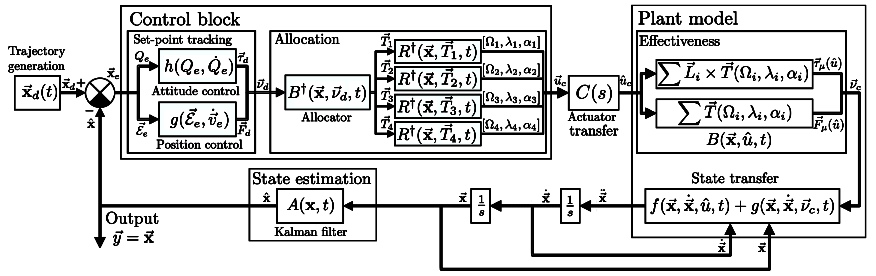
\includegraphics[width=\textwidth]{figs/control-block}
\caption{Extended control loop with overactuation}
\label{fig:control-block}
\vspace{-8pt}
\end{figure}
\par
Certain blocks in Fig:\ref{fig:control-block} use commanded actuator position estimates $\hat{u}_c$ to calculate responses for feedback compensation. In summary, each controller designs either a net force $\vec{F}_d$ for position or a net torque $\vec{\tau}_d$ to act on the body. Allocation rules decompose that virtual input $\vec{\nu}_d$ into four separate 3-D thrust vectors $\vec{T}_{[1:4]}\in\mathbb{R}^{1\times 12}$, or twelve directional components. The force components are an abstracted allocation layer in place of explicit actuator positions, which are subsequently solved for using a static inverse trigonometry.
\begin{equation}
B^{\dagger}(\mathbf{x},\vec{\nu}_d,t)=\big[ T_{1x},~T_{1y},~T_{1z},~\ldots~T_{4x},~T_{4y},~T_{4z}\big]^T
\end{equation}
Each control law is co-dependent on an accompanying allocation algorithm. Traditional control loops (underactuated or well matched) typically have a unity allocation rule and as such require no consideration so they are mostly disregarded. Separate control laws for attitude and position control are presented in Section:\ref{sec:control.attitude} and \ref{sec:control.position} respectively. Thereafter a series of allocation rules are proposed in Ch:\ref{ch:allocation}. Although presented independently, the controller and allocation laws are co-dependent. The stability of each controller is proven in the Lyapunov sense but explicit controller coefficients are optimized in the subsequent Ch:\ref{ch:simulation}, in Sec:\ref{sec:simulation.tuning}.
%====================================================
\section{Stability}
\label{sec:control.stability}
%====================================================
Before undertaking the control plant derivations, it is worth outlining definitions of control stability first. The research question aims to achieve non-zero setpoint tracking of the state's trajectory. A control loop then aims to \emph{stabilize} the closed loop dynamics described previously in Sec:\ref{sec:dynamics.model} whilst tracking particular trajectories for attitude and position setpoints, $\vec{\mathbf{x}}_d(t)=[\vec{\mathcal{E}}_d(t)~Q_d(t)]^T$. 
\par
The entire system's control loop was detailed in Sec:\ref{sec:control.loop}. Stability in the context of trajectory tracking must first be defined. Generalized trajectory stability definitions are not uncommon in the context of energy based control design, or Lyapunov theory (Sec:\ref{sec:control.lyapunov}). Stability definitions pertinent to Lyapunov's stability theorem are briefly presented here, the following is adapted from \cite{lyapunovconference}. In general, for some autonomous trajectory $\vec{\mathbf{x}}(t)$, an equilibrium point at the origin  $\vec{0}$ is said to be stable (\textbf{S}) at $t = t_0$ if and only if (\emph{iff}) the following is true:
\begin{subequations}\label{eq:basic-stability}
\begin{equation}
\forall\varepsilon>0,~\exists~\delta_0(t_0,\varepsilon):~\norm{\vec{\mathbf{x}}(t_0)}<\delta_0(t_0,\varepsilon)
\end{equation}
\vspace{-20pt}
\begin{equation}
\text{and}~\norm{\vec{\mathbf{x}}(t)}<\varepsilon,~~\forall t\geq t_0
\end{equation}
\end{subequations}
The implication of which is that if, for some initial condition $\vec{\mathbf{x}}(t_0)$ whose magnitude is bound by the manifold $\delta_0(t_0,\varepsilon)$, the entire subsequent trajectory of $\vec{\mathbf{x}}(t)$ is bound from above by some other manifold $\varepsilon$. Generalized stability is illustrated in Fig:\ref{fig:basic-stability} for a 2-D trajectory.
\begin{figure}[hbtp]
\vspace{-6pt}
\centering
\begin{subfigure}{0.49\textwidth}
\centering
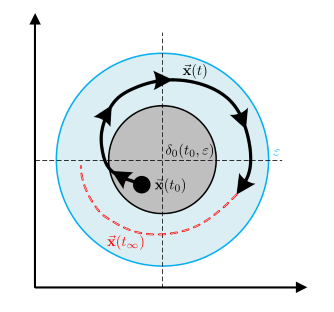
\includegraphics[width=\textwidth]{figs/basic-stability}
\vspace{-16pt}
\caption{Generalized stability}
\label{fig:basic-stability}
\end{subfigure}
\begin{subfigure}{0.49\textwidth}
\centering
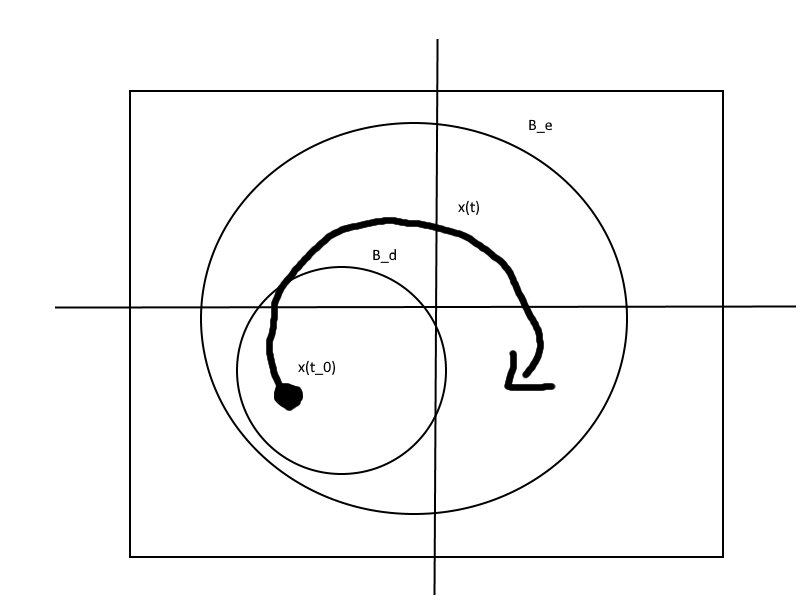
\includegraphics[width=\textwidth]{figs/uniform-stability}
\vspace{-16pt}
\caption{Uniform stability}
\label{fig:uniform-stability}
\end{subfigure}
\vspace{-8pt}
\caption{Trajectory illustrations for $\mathbf{S}$ and $\mathbf{US}$}
\vspace{-18pt}
\end{figure}
\par
An equilibrium point is further said to be uniformly stable (\textbf{US}) \emph{iff} for the time $t\in[t_0,\infty)$ the following criteria, being an extension of general stability, are met:
\begin{subequations}\label{eq:uniform-stability}
\begin{equation}
\forall\varepsilon>0,~\exists~\delta_0(\varepsilon)>0:~\norm{\vec{\mathbf{x}}(t_1)}<\delta_0(\varepsilon),~~t_1>t_0
\end{equation}
\vspace{-18pt}
\begin{equation}
\text{and}~\norm{\vec{\mathbf{x}}(t)}<\varepsilon,~~\forall
t\geq t_1
\end{equation}
\end{subequations}
\textbf{US} similarly bounds a trajectory from above by $\varepsilon$ if the trajectory originates from within $\delta_0(\varepsilon)$. The difference is that the principle trajectory region $\delta_0(\varepsilon)$ is independent of $t_0$ in the case of \textbf{US}.
\par
The two surfaces are non-concentric, a $\mathbf{US}$ trajectory is illustrated in Fig:\ref{fig:uniform-stability}. Uniform stability is a subset of general stability, $\mathbf{US}\subset\mathbf{S}$, however the converse is not true. Furthermore \textbf{US} is a stronger qualification of stability, each subsequent stability presented represents a stronger assertion of stability.
\par
Extending stability definitions to include settling, an equilibrium point is said to be asymptotically stable (\textbf{AS}) \emph{iff} conditions for \textbf{S} are met (Eq:\ref{eq:basic-stability}) and that the following holds true:
\begin{subequations}\label{eq:asymptotic-stability}
\begin{equation}
\exists~\delta_1(t_0,\varepsilon) >0:~\norm{\vec{\mathbf{x}}(t_0)}<\delta_1(t_0,\varepsilon)
\end{equation}
\vspace{-18pt}
\begin{equation}
\text{and}~\lim_{t\rightarrow\infty}\norm{\vec{\mathbf{x}}(t)}\rightarrow 0
\end{equation}
\end{subequations}
This asserts that trajectories originating within some finer region $\delta_1(t_0,\varepsilon)$, being a subset of $\delta_0(t_0,\varepsilon)$, tend to and \emph{asymptotically} settle at the origin. In the case of \textbf{AS} the origin is both \emph{stable} and \emph{attractive} (shown in Fig:\ref{fig:asymptotic-stability}). Asymptotic stability is typically the first requirement for any control law, being a stronger stability than both \textbf{US} and \textbf{S}, typically stabilizing a control setpoint's error.
\begin{figure}[hbtp]
\centering
\begin{subfigure}{0.49\textwidth}
\centering
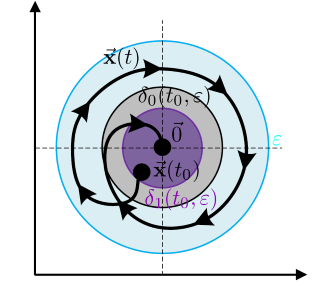
\includegraphics[width=\textwidth]{figs/asymptotic-stability}
\vspace{-8pt}
\caption{Asymptotic stability}
\label{fig:asymptotic-stability}
\end{subfigure}
\begin{subfigure}{0.49\textwidth}
\centering
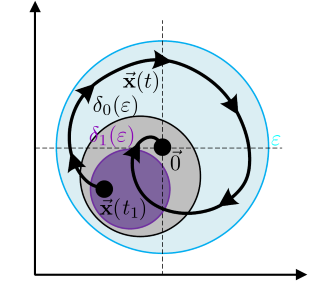
\includegraphics[width=\textwidth]{figs/uniform-asymptotic-stability}
\vspace{-8pt}
\caption{Uniform asymptotic stability}
\label{fig:uniform-asymptotic-stability}
\end{subfigure}
\vspace{-4pt}
\caption{Trajectory illustrations for $\mathbf{AS}$ and $\mathbf{UAS}$}
\vspace{-14pt}
\end{figure}
\par
Uniform asymptotic stability (\textbf{UAS}), an extension of asymptotic stability $\mathbf{UAS}\subset\mathbf{AS}$, occurs when the asymptotically stable bound region $\delta_1(\varepsilon)$ is independent of the principle starting time $t_0$. An equilibrium point is \textbf{UAS} \emph{iff} conditions for \textbf{S} are met and that:
\begin{subequations}\label{eq:uniform-asymptotic-stability}
\begin{equation}
\exists~\delta_1(\varepsilon)>0:~\norm{\vec{\mathbf{x}}(t_1)}<\delta_1(\varepsilon),~~t_1\geq t_0
\end{equation} 
\vspace{-16pt}
\begin{equation}
\text{and}~\lim_{t\rightarrow\infty}\norm{\vec{\mathbf{x}}(t)}\rightarrow 0
\end{equation}
\end{subequations}
A uniformly asymptotic equilibrium point implies a stable trajectory starting within a non-concentric region, independent of the starting time $t_0$, and settling to the origin (illustrated in Fig:\ref{fig:uniform-asymptotic-stability}). 
\par
A trajectory is regarded as exponentially stable (\textbf{UES}) if conditions for \textbf{UAS} are met and that there exist $\exists~a,b,r$ that bound the settling of the trajectory such that:
\begin{equation}\label{eq:exponential-stability}
\norm{\vec{\mathbf{x}}(t,t_0,\vec{\mathbf{x}}_0)}\leq a\norm{\vec{\mathbf{x}}_0}e^{-bt},~~\forall\norm{\vec{\mathbf{x}}_0}\leq r
\end{equation}
The term $a\norm{\vec{\mathbf{x}}_0}e^{-bt}$ bounds the worst case rate at which the trajectory settles to the origin, illustrated in Fig:\ref{fig:exponential-stability}. Exponential stability guarantees that the magnitude displacement of the trajectory at any given point in time is less than an explicit exponential decay. The initial point of the trajectory, $\vec{\mathbf{x}}_0$, is bound from above by some $r\triangleq \delta_1(\varepsilon)$. Moreover uniform stability is \emph{implied} with exponential stability.
\newpage
\begin{figure}[hbtp]
\centering
\begin{subfigure}{0.49\textwidth}
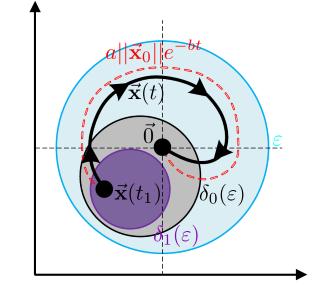
\includegraphics[width=\textwidth]{figs/exponential-stability}
\vspace{-14pt}
\caption{Exponential stability}
\label{fig:exponential-stability}
\end{subfigure}
\begin{subfigure}{0.49\textwidth}
\centering
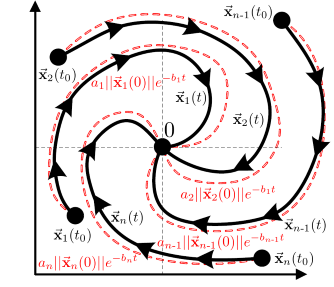
\includegraphics[width=\textwidth]{figs/global-exponential-stability}
\vspace{-14pt}
\caption{Global exponential stability}
\label{fig:global-exponential-stability}
\end{subfigure}
\vspace{-2pt}
\caption{Trajectory illustrations for \textbf{UES} and \textbf{GUES}}
\vspace{-6pt}
\end{figure}
The above definitions of stabilities are only locally defined, and so the stabilities hold true only for local trajectories, only in the case of $\vec{\mathbf{x}}(t_0)\leq\varepsilon$. Extending \textbf{UAS} to global uniform asymptotic stability (\textbf{GUAS}), the origin's equilibrium point is \textbf{GUAS} \emph{iff} conditions for \textbf{UAS} are first met, the origin is only the equilibrium point and the asymptotic approach can be extended such that:
\begin{subequations}
\begin{equation}
\exists~\delta_1(\varepsilon)>0:~\norm{\vec{\mathbf{x}}(t_1)}<\delta_1(\varepsilon),~~t_1\geq t_0
\end{equation}
\vspace{-16pt}
\begin{equation}
\text{and}~ \lim_{t\rightarrow\infty}\norm{\vec{\mathbf{x}}(t)}\rightarrow 0,~~\forall \vec{\mathbf{x}}(t_0)
\end{equation}
\end{subequations}
Similarly, exponential stability can extend to the global case, shown in Fig:\ref{fig:global-exponential-stability}, but only \emph{iff} \textbf{UES} conditions are first met. In the global case, the origin can be the \emph{only equilibrium point}. Stability from Eq:\ref{eq:exponential-stability} is then globally:
\begin{equation}\label{eq:global-exponential-stability}
\norm{\vec{\mathbf{x}}(t,t_0)}\leq a\norm{\vec{\mathbf{x}}_0}e^{-bt},~~\forall\norm{\vec{\mathbf{x}}_0}
\end{equation}
Initial trajectory conditions are dropped in Eq:\ref{eq:global-exponential-stability} for any number of trajectories until $\vec{\mathbf{x}}_n(t)$ each trajectory is bound by an exponential $a_n\norm{\vec{\mathbf{x}}_t(0)}e^{-b_nt}$. It follows that, irrespective of the starting point $\vec{\mathbf{x}}_n(t_0)$ for the trajectory, the system \emph{always} settles to the origin. \textbf{GUES} is the strongest sense of stability and provides insight into the trajectory stabilizing rate. The most desirable control design outcome is a controller which applies globally uniform exponential stability to a plant.
%====================================================
\section{Lyapunov Stability Theory}
\label{sec:control.lyapunov}
%====================================================
Lyapunov's stability theory is an important aspect of nonlinear controller design. If the reader is unfamiliar with Lyapunov's theorem,  \cite{noteonlyapunov,nonlinearsystems,bojelayupanov} each provide thorough explanations of the concept. The following is adapted from \cite{lyapunovconference} and \cite{lyapunovpaper} and briefly outlines how Lyapunov's stability theory is used to prove (\emph{global}) asymptotic stability for continuous time invariant systems, linear or otherwise. 
\par
The theory analyzes a generalized energy function of a system's autonomous trajectory, if the trajectory has a negative energy derivative that implies the system's energy will always dissipate towards a state of zero energy or stable equilibrium point. Lyapunov analysis is a powerful tool for stability verification because the system's trajectory itself need not be explicitly defined for stability to be determined. It is worth reiterating Lyapunov fundamentals given that backstepping controllers are proposed later in Sec:\ref{subsec:control.attitude.nonlinear} for attitude control.
\newpage
A backstepping controller enforces Lyapunov stability criteria onto the system through iterative control structure design, \cite{backstepping,adaptivebackstep,intelligentbackstep}. In general, given a nonlinear time invariant system that follows some continually differentiable trajectory $\vec{\mathbf{x}}(t)$, typically the trajectory is going to progress subject to some autonomous rule:
\begin{equation}\label{eq:4.17}
\dot{\vec{\mathbf{x}}}(t)=f\big(\vec{\mathbf{x}}(t)\big)
\end{equation}
Then a generalized positive-definite function generalized energy or \emph{Lyapunov function candidate} (\emph{LFC}) $V(\vec{\mathbf{x}})$ for a trajectory $\vec{\mathbf{x}}(t)$ is constructed. A positive definite matrix $M$ is defined such that:
\begin{equation}
\mathbf{z}^TM\mathbf{z} > 0~~~\forall \mathbf{z}\not = 0
\end{equation}
As such an LFC typically, but not exclusively, has the quadratic and positive-definite form with some positive square matrix $P\in\mathbb{R}^{n\times n}>0$:
\begin{equation}
V(\vec{\mathbf{x}})=\vec{\mathbf{x}}\hspace{1pt}^TP\vec{\mathbf{x}},~~\vec{\mathbf{x}}\in\mathbb{R}^{n}
\end{equation}
An LFC could simply be positive semi-definite over the trajectory's path, the quadratic form is just convenient for the use of backstepping. From its definition the trajectory Eq:\ref{eq:4.17} is continually differentiable, there is then a gradient matrix for each element of $V(\vec{\mathbf{x}})$ in the form:
\begin{equation}\label{eq:4.20}
\nabla V(\vec{\mathbf{x}})\triangleq\bigg[\frac{\partial V(\vec{\mathbf{x}})}{\partial x_1}~\frac{\partial V(\vec{\mathbf{x}})}{\partial x_2}~\ldots~\frac{\partial V(\vec{\mathbf{x}})}{\partial x_n}\bigg]~~~~\vec{\mathbf{x}}\in\mathbb{R}^n
\end{equation}
The energy function's derivative, otherwise referred to as the \emph{Lie derivative}, is calculated from partial derivatives in Eq:\ref{eq:4.20} as follows:
\begin{equation}\label{eq:lyapunov-derivative}
\dot{V}(\vec{\mathbf{x}})\triangleq\nabla V(\vec{\mathbf{x}})^Tf(\vec{\mathbf{x}})=\frac{\partial V(\vec{\mathbf{x}})}{\partial x_1}f_1(x_1)+\frac{\partial V(\vec{\mathbf{x}})}{\partial x_2}f_2(x_2)+~\ldots~+\frac{\partial V(\vec{\mathbf{x}})}{\partial x_n}f_n(x_b)
\end{equation}
Lyapunov's theorem states that if the candidate function $V(\vec{\mathbf{x}})$ is positive definite with $V(\vec{0})=0$ and its derivative is strictly negative, $\dot{V}(\vec{\mathbf{x}})< 0~~\forall \vec{\mathbf{x}}(t) \not= 0$, the system has global uniform asymptotic stability ($\mathbf{GUAS}$ from Eq:\ref{eq:asymptotic-stability}). Mathematically that means, for any $\vec{\mathbf{x}}(t)$ with $t\geq t_0$:
\begin{equation}\label{eq:4.22}
V\big(\vec{\mathbf{x}}(t)\big)=V\big(\vec{\mathbf{x}}(t_0)\big)+\int_{t_0}^t \dot{V}\big(\vec{\mathbf{x}}(t)\big).dt \leq V\big(\vec{\mathbf{x}}(t_0)\big)
\end{equation}
which can be physically interpreted as the system's generalized energy (function) dissipating, irrespective of the trajectory path taken. With a strictly decreasing energy function, the system will stabilize to a state of zero energy which, naturally, is a stable equilibrium point.
\begin{equation}
\lim_{t\rightarrow\infty}\norm{V\big(\vec{\mathbf{x}}(t)\big)}\rightarrow 0
\end{equation}
The trajectory's asymptotic stability can be extended to exponential stability boundedness, such that if the same conditions are met for asymptotic stability in Eq:\ref{eq:4.22} and there exists some positive coefficient $\alpha>0$ such that $\dot{V}(\vec{\mathbf{x}})<-\alpha V(\vec{\mathbf{x}})$. That implies the system is globally exponentially stable and is bound in such a way that:
\begin{equation}\label{eq:lyapunov-exponential-stability}
\norm{V\big(\vec{\mathbf{x}}(t)\big)}\leq Me^{-\alpha}\norm{V\big(\vec{\mathbf{x}}(t_0)\big)}
\end{equation}
%====================================================
\section{Model Dependent \& Independent Controllers}
%====================================================
Two classes of controllers are included for the trajectory tracking control loop, both attitude and position control laws. Attitude setpoint tracking is the primary focus of this research project (Sec:\ref{subsec:control.attitude.problem}) and incorporates a more detailed schedule of controller design and evaluation. The allocation law combines both virtual control inputs from attitude and position controllers, $\vec{\nu}_d=[\vec{F}_d~\vec{\tau}_d]^T$, to solve for explicit actuator positions. 
\par
Controller dependency on the plant's state is as a consequence of the actuator responses and complex inertial dynamics, as derived previously in Sec:\ref{subsec:dynamics.nonlinearities.gyrotorques}. Whilst not a prerequisite for stability, plant dependent compensation obviously improves controller performances. Independent and dependent cases are only considered for one type of controller, the most basic case proportional-derivative controller in Section:\ref{subsubsec:control.attitude.controllers.pd} and tested in Sec:\ref{subsec:simulation.attitude.pd}. All other control laws compensate for unwanted plant dynamics in a feedback configuration.
\par
The plant dependency makes backstepping controllers an effective controller choice for this dissertation's context. The proposed plant dependent control laws compensate for undesirable dynamics by design, basic PD and PID control structures (\emph{and the like}) will not. The first and most basic control solution, used as a reference case, is a PD controller for attitude and position with direct-inversion (Pseudo or Moore-Penrose inversion) allocation. 
%====================================================
\section{Attitude Control}
\label{sec:control.attitude}
%====================================================
\subsection{The Attitude Control Problem}
\label{subsec:control.attitude.problem}
%====================================================
The setpoint tracking control problem for the attitude plant\cite{attitudecontrolproblem}, is to design a stabilizing control torque $\vec{\tau}_d=h(\vec{\mathbf{x}}_e,\dot{\vec{\mathbf{x}}}_e,t)$ such that for any desired attitude quaternion $\forall~Q_d\in\mathbb{Q}$ and an instantaneous attitude body quaternion $Q_b\in\mathbb{Q}$, the error state asymptotically stabilizes to the origin $Q_e\rightarrow[\pm 1~\vec{0}~]^T$. Or that:
\begin{equation}\label{eq:quaternion-attitude-problem}
\vec{\tau}_d=h(Q_d,~\dot{Q}_d,~Q_b,~\dot{Q}_b)~~\text{such that}~~\underset{t\rightarrow\infty}{\lim}Q_b\rightarrow Q_d
\end{equation}
Quaternion attitude error states are defined as the Hamilton product or \emph{difference} between the desired and instantaneous quaternion attitude states, previously in Eq:\ref{eq:quaternion-error}. Quaternion error states are multiplicative, in contrast to the subtractive relationship for Euler angle error states. The attitude error state is defined as:
\begin{equation}\label{eq:quaternion-error-control}
Q_e\triangleq Q_b^*\otimes Q_d
\end{equation}
The relative angular velocity error between the body frame $\mathcal{F}^b$ and the trajectory's desired frame $\mathcal{F}^d$ is given as $\vec{\omega}_e$. The desired angular velocity $\vec{\omega}_d$ is taken with respect to the desired angular attitude frame $\mathcal{F}^{d}$, and therefore must be first transformed back to the existing body frame.
\begin{subequations}
\begin{equation}\label{eq:angular-error}
\vec{\omega}_e\triangleq Q_e^*\otimes\vec{\omega}_d\otimes Q_e-\vec{\omega}_b~~~~\in\mathcal{F}^{b}
\end{equation}
For the trajectories generated here, only first order setpoints are commanded, hence the desired angular velocity is zero or that $\vec{\omega}_d\triangleq\vec{0}$. It follows that the angular velocity error is then simply the negative body angular velocity. It would be easy to incorporate a non-zero angular velocity setpoint to accommodate for higher order state derivative tracking trajectories.
\begin{equation}\label{eq:4.27c}
\therefore\vec{\omega}_e=-\vec{\omega}_b\Big|_{\vec{\omega}_d=\vec{0}}
\end{equation}
\end{subequations}
The time derivative for the quaternion error state is calculated from the quaternion rate definition in Eq:\ref{eq:quaternion-deriv}. The quaternion error derivative $\dot{Q}_e$ depends on the angular velocity error and is calculated:
\begin{equation}
\dot{Q}_e=\frac{1}{2}Q_e\otimes\vec{\omega}_e=-\frac{1}{2}Q_e\otimes\vec{\omega}_b\Big|_{\vec{\omega}_d=\vec{0}}
\end{equation}
Stability proofs for each of the subsequent controllers apply Lyapunov stability theory to analyze the attitude quaternion error's  trajectory. If the attitude error is asymptotically stabilized, it follows that the attitude state will track its setpoint, Eq:\ref{eq:quaternion-attitude-problem}. Typically, proposed Lyapunov Function candidates for a quaternion error trajectory all take the standard quadratic form:
\begin{equation}\label{eq:lyapunov-quaternion}
V(Q_e)=\vec{q}_e\text{}^T\vec{q}_e+(1-q_0)^2
\end{equation}
For Lyapunov's stability theory to be applied, a valid Lyapunov function candidate \emph{must} be positive definite. The constraints on the quaternion trajectory LFC in Eq:\ref{eq:lyapunov-quaternion} are that $V(Q_e)>0~~\forall(Q_e)\not = 0$ and that it must be zero at the origin (in this case a zero quaternion $Q_e=[\pm 1~\vec{0}\hspace{2pt}]^T$) so the requirement is that $V([\pm1~\vec{0}\hspace{2pt}])=0$. Unless a variable substitution is performed for the quaternion attitude error, the Lyapunov function candidate Eq:\ref{eq:lyapunov-quaternion} is only positive definite for a local quaternion trajectory with $q_0\in[0:1]$. A variable substitution presented in \cite{satellitebackstepping} replaces the quaternion scalar with its absolute value, to be used as a backstepping state variable:
\begin{subequations}
\begin{equation}
z_1\triangleq \begin{bmatrix}
1-|q_0|\\
\vec{q}_e
\end{bmatrix}
\end{equation}
which is then used as a trajectory variable in the \emph{positive definite} Lyapunov function candidate:
\begin{equation}
V(z_1)=z_1^Tz_1>0~~\forall z_1\not = 0
\end{equation}
\end{subequations}
Substitution for a quaternion scalar's absolute value makes the control law more complicated when trying to enforce backstepping iteration, shown next in Sec:\ref{subsubsec:control.attitude.nonlinear.idealbackstep}. Alternatively, limiting the quaternion error's scalar to a range $q_0\in[0:1]$ reduces the ``dual-coverage" quaternions have of $R^3$ attitudes when described in $R^4$ space. If one considers how an error quaternion relates to an Euler-axis rotation of an error angle $\theta_e$ about an error unit axis $\hat{u}_e$, from the definition of a quaternion in Eq:\ref{eq:quaternion-euler-axis}:
\begin{equation}
Q_e=\begin{bmatrix}
q_0\\
\vec{q}_e
\end{bmatrix}
\triangleq
\begin{bmatrix}
cos(\theta_e/2)\\
sin(\theta_e/2)\hat{u}_e
\end{bmatrix}
\end{equation}
then a constraint applied to $q_0\in[0:1]$ limits the Euler-axis error rotation $\theta_e\in[-\pi:\pi]$. In practical terms the stability proofs for such a limited quaternion trajectory \emph{will not} guarantee global stability in the quaternion space $\mathbb{R}^4$, \emph{but} it will guarantee global 3-D stability in SO(3) or $\mathbb{R}^3$. That is not to say a particular controller cannot be stable for the full $q_0\in[-1:1]$, the stability is only \emph{guaranteed} for the constrained range. Because $Q=[\pm q_0~\vec{q}\hspace{2pt}]$ corresponds to the same physical attitude in $\mathbb{R}^{3}$, the calculated quaternion error $Q_e$, from Eq:\ref{eq:quaternion-error-control}, can be constrained with an absolute value quaternion scalar without limiting the rigid body attitude plant. Using the definition for quaternion multiplication in Eq:\ref{eq:quaternion-product} and the quaternion conjugate in Eq:\ref{eq:quaternion-conjugate}, the quaternion error is refined:
\begin{equation}\label{eq:constrained-quaternion-error}
Q_e = \begin{bmatrix}
q_0\\
\vec{q}_e
\end{bmatrix}
\triangleq
\begin{bmatrix}
|q_{b0}q_{d0}+\vec{q}_b\cdot\vec{q}_d|\\
q_{b0}\vec{q}_d-q_{d0}\vec{q}_b-\vec{q}_b\times\vec{q}_d
\end{bmatrix}
\end{equation}
Using the constrained quaternion in Eq:\ref{eq:constrained-quaternion-error} for control calculations then ensures that global stability of the rigid body's attitude in $\mathbb{R}^3$ can be guaranteed by the subsequent stability proofs. Neither the angular velocity error $\vec{\omega}_e$, nor the quaternion error derivative $\dot{Q}_e$, both in Eq:\ref{eq:4.27c}, are affected by the refinement.
%====================================================
\subsection{Linear Controllers}
\label{subsec:control.attitude.controllers}
%====================================================
\subsubsection{PD Controller}
\label{subsubsec:control.attitude.controllers.pd}
%====================================================
The following control law is used as a reference case for comparing the subsequent designed controllers. It is a simple proportional-derivative (\emph{PD}) attitude controller, adapted from \cite{fullquaternion} and applies a stability proof similar to the one derived in \cite{attitudecontrolproblem}. An attitude PD controller is proportional only to the \emph{vector quaternion error}, so that the error is then of the same dimension as the angular velocity error, $\vec{q}_e\in\mathbb{R}^3$. A PD controller generates the commanded torque input:
\begin{equation}\label{eq:independent-pd}
\vec{\tau}_{_{PD}}=J_b(u)\big(K_d\vec{\omega}_e+K_p\vec{q}_e\big)~~~~\in\mathcal{F}^b
\end{equation}
where both $K_d$ and $K_p$ are \emph{positive symmetrical} $3\times 3$ gain coefficient matrices to be determined at a later stage.
\par
Positive symmetry imposed on the coefficients in Eq:\ref{eq:independent-pd} simplifies the stability proof that follows but is not necessarily a prerequisite. Because Eq:\ref{eq:independent-pd} neglects the quaternion scalar error, it is therefore susceptible to unwinding. Using a positive-definite Lyapunov function candidate $V_{_{PD}}$ for the attitude trajectory:
\begin{equation}\label{eq:lyapunov-pd}
V_{_{PD}}(Q_e,\vec{\omega}_e)\triangleq\vec{q}_e\text{}^T\vec{q}_e+(1-q_0)^2+\frac{1}{2}\vec{\omega}_e\text{}^TK_p^{-1}\vec{\omega}_e>0~~\forall(Q_e,\vec{\omega}_e)\not = \vec{0}
\end{equation}
The origin is an equilibrium point as a result of the constrained quaternion error trajectory proposed in Eq:\ref{eq:constrained-quaternion-error}. Then $V_{_{PD}}([1~\vec{0}\hspace{1pt}]^T,\vec{0}\hspace{1pt})=0$, which makes it positive definite and a suitable Lyapunov function candidate. Exploiting the unit quaternion's inherent magnitude property:
\begin{equation}\label{eq:4.171}
\norm{Q}\triangleq\vec{q}\text{}^{\hspace{3pt}T}\vec{q}+q_0\text{}^2=\vec{q}\text{}^{\hspace{3pt}2}+q_0\text{}^2=1
\end{equation}
and substituting the unit quaternion's identity and the angular velocity's error state $\vec{\omega}_e=-\vec{\omega}_b$, the proportional derivative LFC from Eq:\ref{eq:lyapunov-pd} reduces to:
\begin{subequations}\label{eq:4.18}
\begin{equation}
V_{_{PD}}=\vec{q}_e\text{}^2+\big(q_0\text{}^2 -2q_0 + 1\big) +\frac{1}{2}\vec{\omega}_e\text{}^TK_p^{-1}\vec{\omega}_e
\end{equation}
\vspace{-10pt}
\begin{equation}
=2(1-q_0)+\frac{1}{2}\vec{\omega}_b\text{}^TK_p^{-1}\vec{\omega}_b\Big|_{\vec{\omega}_e=-\vec{\omega}_b}
\end{equation}
\end{subequations}
Taking the derivative of that Lyapunov Function candidate then yields:
\begin{equation}\label{eq:lyapunov-pd-deriv}
\dot{V}_{_{PD}}(Q_e,\vec{\omega}_e)=-2\dot{q}_0+\vec{\omega}_b\text{}^TK_p^{-1}\dot{\vec{\omega}}_b
\end{equation}
Then, using the error quaternion's derivative $\dot{Q}_e$ and noting that $\vec{\omega}_e=-\vec{\omega}_b$:
\begin{subequations}
\begin{equation}\label{eq:control-quat-derivative}
\dot{Q}_e\triangleq\begin{bmatrix}
-\frac{1}{2}\vec{q}_e\text{}^T\vec{\omega}_e\\
\frac{1}{2}\big([\vec{q}_e]_\times+q_0\mathbb{I}_{3\times 3}\big)\vec{\omega}_e
\end{bmatrix}
\end{equation}
\vspace{-6pt}
\begin{equation}
=-\frac{1}{2}\begin{bmatrix}
-\vec{q}_e\text{}^T\vec{\omega}_b\\
\big([\vec{q}_e]_\times+q_0\mathbb{I}_{3\times 3}\big)\vec{\omega}_b
\end{bmatrix}
\end{equation}
Substituting the error quaternion's scalar derivative $\dot{q}_0$ back into the LFC derivative Eq:\ref{eq:lyapunov-pd-deriv} gives:
\begin{equation}\label{eq:control-angular}
\therefore\dot{V}_{_{PD}}=-\vec{q}_e\text{}^T\vec{\omega}_b+\vec{\omega}_b^TK_P^{-1}\dot{\vec{\omega}}_b
\end{equation}
\end{subequations}
Recalling the angular velocity differential equation from Eq:\ref{eq:quaternion-states-angular} for $\dot{\vec{\omega}}_b$ with a control torque input $\vec{\tau}_{_{PD}}$ from Eq:\ref{eq:independent-pd}:
\begin{subequations}
\begin{equation}
\dot{\vec{\omega}}_b=J_b\text{}^{-1}(u)\big(-\vec{\omega}_b\times J_b(u)\vec{\omega}_b-\vec{\tau}_b(u)+\vec{\tau}_g+\vec{\tau}_H+\vec{\tau}_{_{PD}}\big)~~~~\in\mathcal{F}^b
\end{equation}
Using the definition of the proportional derivative torque control law from Eq:\ref{eq:independent-pd}, the angular acceleration equation Eq:\ref{eq:control-angular} for $\dot{\vec{\omega}}_b$ becomes:
\begin{equation}
\dot{\vec{\omega}}_b=J_b\text{}^{-1}(u)\big(-\vec{\omega}_b\times J_b(u)\vec{\omega}_b-\vec{\tau}_b(u)+\vec{\tau}_g+\vec{\tau}_H\big)-K_d\vec{\omega}_b+K_p\vec{q}_e
\end{equation}
\end{subequations}
Substituting the above into the LFC derivative $\dot{V}_{_{PD}}$ in Eq:\ref{eq:lyapunov-pd-deriv} yields:
\begin{subequations}
\begin{equation}
\dot{V}_{_{PD}}=-\vec{q}_e\text{}^T\vec{\omega}_b+\vec{\omega}_b\text{}^TK_p^{-1}\Big(-K_d\vec{\omega}_b+K_p\vec{q}_e+J_b^{-1}(u)\big(-\vec{\omega}_b\times J_b(u)\vec{\omega}_b-\vec{\tau}_b+\vec{\tau}_g+\vec{\tau}_H\big)\Big)
\end{equation}
\vspace{-18pt}
\begin{equation}
=-\vec{q}_e\text{}^T\vec{\omega}_b+\vec{\omega}_b\text{}^T\vec{q}_e-\vec{\omega}_b\text{}^TK_p^{-1}K_d\vec{\omega}_b+\vec{\omega}_b\text{}^T\Big(K_pJ_b(u)\Big)^{-1}\big(-\vec{\omega}_b\times J_b(u)\vec{\omega}_b-\vec{\tau}_b(u)+\vec{\tau}_g+\vec{\tau}_H\big)
\end{equation}
The transposed terms $\vec{q}_e\text{}^T\vec{\omega}_b ~\text{and}~\vec{\omega}_b\text{}^T\vec{q}_e$ are interchangeable so then $-\vec{q}_e\text{}^T\vec{\omega}_b+\vec{\omega}_b\text{}^T\vec{q}_e=0$. The LFC derivative $\dot{V}_{_{PD}}$ then simplifies to:
\begin{equation}\label{eq:independent-lyapunov-derivative}
\dot{V}_{_{PD}}=-\vec{\omega}_b\text{}^TK_p^{-1}K_d\vec{\omega}_b+\vec{\omega}_b\text{}^T\Big(K_pJ_b(u)\Big)^{-1}\big(-\vec{\omega}_b\times J_b(u)\vec{\omega}_b-\vec{\tau}_b(u)+\vec{\tau}_g+\vec{\tau}_Q\big)
\end{equation}
\end{subequations}
Then, as long as the enitre term $\big(-\vec{\omega}_b\times J_b(u)\vec{\omega}_b-\vec{\tau}_b(u)+\vec{\tau}_g+\vec{\tau}_Q\big)$ is negative semi-definite or $<\vec{0}$, some element of stability is can be achieved. Under specific circumstances the following assumptions can be made to apply an asymptotic stability proof:
\vspace{-10pt}
\begin{enumerate}[itemsep=0em]
\item The inertia matrix $J_b(u)$ is approximately diagonal, which, given the inertia eigenvalues from Eq:\ref{eq:inertia-max} and Eq:\ref{eq:inertia-min}, is reasonable. Similarly, the angular velocity can be made small with an appropriately slow trajectory such that the torque gyroscopic cross-product is negligible:
\begin{center}
\vspace{-10pt}
$\big(-\vec{\omega}_b\times J_b(u)\vec{\omega}_b\big)\approx\vec{0}$
\vspace{-8pt}
\end{center}
\item The actuator rate torque response, $\vec{\tau}_b(u)$, is a second order effect dependent on $d\vec{u}/dt$. Typically the actuator rates are going to be kept small. For small actuator step changes the inertia rates of change and servo accelerations in Eq:\ref{eq:actuator-torque} are small enough to be considered negligible. The assumption is then made:
\begin{center}
\vspace{-10pt}
$\vec{\tau}_b(u)\approx\vec{0}$
\vspace{-8pt}
\end{center}
\item Finally, for the sake of the stability proof, the eccentric gravitational torque arm, from a varying center of gravity $\Delta\vec{C}_G$, from Eq:\ref{eq:consolidated-grav-torque}, is neglected. Such a situation only holds true if $\vec{u}\approx\vec{0}$ or that servo actuator positions are close to their zero positions.
\begin{center}
\vspace{-10pt}
$\vec{\tau}_g\approx\vec{0}$
\vspace{-8pt}
\end{center}
\end{enumerate}
All of the above assumptions are made under extraneous circumstances, the subsequent stability obviously breaks down if any of assumptions 1 through 3 fail. Stability achieved using the above plant \emph{independent} control law is only local, and will not hold true for most of the prototype's flight envelope, which involves time varying angular velocities $\vec{\omega}_b\not = \vec{0}$. 
\par
The plant independent case is considered and simulated in Sec:\ref{subsubsec:simulation.atttiude.pd.independent} only to demonstrate the need for plant dependent compensation. If each of the assumptions hold true, then the unwanted dynamic terms in Eq:\ref{eq:independent-lyapunov-derivative} are negligible or $\big(-\vec{\omega}_b\times J_b(u)\vec{\omega}_b-\vec{\tau}_b(u)+\vec{\tau}_g+\vec{\tau}_Q\big)\approx 0$, resulting in a negative definite Lyapunov function derivative. The stability proof for that very local trajectory is then:
\begin{subequations}
\begin{equation}
\dot{V}_{_{PD}}=-\vec{q}_e\text{}^T\vec{\omega}_b+\vec{\omega}_b\text{}^TK_p^{-1}\big(-K_d\vec{\omega}_b+K_p\vec{q}_e\big)
\end{equation}
\vspace{-14pt}
\begin{equation}
=-\vec{\omega}_b\text{}^TK_p^{-1}K_d\vec{\omega}_b
\end{equation}
\vspace{-14pt}
\begin{equation}\label{eq:pd-local-stability}
=-K_p^{-1}K_d\norm{\vec{\omega}_b}\text{}^2<0~~\forall(\vec{q}_e,\vec{\omega}_e),~~q_0\in[0:1],~~\exists~(K_p^{-1},K_d)>0
\end{equation}
\end{subequations}
From Lyapunov stability theorem there then exist the following limits: 
\begin{subequations}
\begin{equation}
\lim_{t\rightarrow\infty}\vec{\omega}_e\rightarrow\vec{0}~~\therefore~~\lim_{t\rightarrow\infty}\vec{\omega}_b\rightarrow\vec{0}
\end{equation}
\vspace{-14pt}
\begin{equation}
\lim_{t\rightarrow\infty}\vec{q}_e\rightarrow \vec{0}~~\text{and}~~\lim_{t\rightarrow\infty}(1-q_0)\rightarrow 0
\end{equation}
\end{subequations}
If $q_0\in[0:1]$ then the quaternion error stabilizes $Q_e\rightarrow[1~\vec{0}\hspace{3pt}]^{T}$ as $t\rightarrow\infty$. The stability shown in Eq:\ref{eq:pd-local-stability} is only local. Introducing plant dependent compensation to the PD control law in Eq:\ref{eq:independent-pd} alleviates the stringent requirements on assumptions 1 through 3, as shown subsequently. Adding compensation terms for the unwanted plants dynamics: 
\begin{equation}\label{eq:dependent-pd}
\vec{\tau}_{_{PD}}=\underbrace{J_b(\hat{u})\big(K_p\vec{q}_e+K_d\vec{\omega}_e\big)}_{\text{Independent}}+\underbrace{\hat{\omega}_b\times J_b(\hat{u})\hat{\omega}_b+\vec{\tau}_b(\hat{u})-\vec{\tau}_g-\vec{\tau}_Q}_{\text{Compensation}}
\end{equation}
Obviously, controller errors and compensation terms rely on \emph{state estimates}, whereas inertias and torque responses are calculated using sampled $\hat{u}_c$ commanded actuator positions. Moreover, the quaternion attitude and angular velocity states $\hat{Q}_b$ and $\hat{\omega}_b$ are both estimates and so a small degree of uncertainty exists. Robust stability in the case of plant dependent uncertainty is investigated in Sec:\ref{sec:simulation.disturbance}, but for now the estimates are \emph{assumed to be free of errors and dynamics}. The resultant stability proof for the plant dependent case, Eq:\ref{eq:dependent-pd}, is much the same as that for the independent controller, Eq:\ref{eq:independent-pd}. The same LFC from Eq:\ref{eq:lyapunov-pd} shows that Eq:\ref{eq:pd-local-stability} holds globally:
\begin{subequations}\label{eq:dependent-global-stability}
\begin{equation}\label{eq:4.40a}
\dot{V}_{_{PD}}=-\vec{\omega}_b\text{}^TK_p^{-1}K_d\vec{\omega}_b
\end{equation}
\vspace{-8pt}
\begin{equation}\label{eq:4.40b}
\therefore \dot{V}_{_{PD}}\leq -K_pK_d\norm{\vec{\omega}_b}\text{}^2<0~~\forall(q_e,\vec{\omega}_e),~~q_0\in[0:1],~~\exists~(K_p^{-1},K_d)>0
\end{equation}
\end{subequations}
The inverse qualifier of $K_p^{-1}$ in Eq:\ref{eq:4.40a} is redundant given that $K_p$ is a symmetrical coefficient matrix. The plant dependent controller compensates for the unwanted dynamics which the independent control otherwise assumes are inconsequential to achieve the same stability. Dynamic compensation in Eq:\ref{eq:dependent-pd} is simple to implement, considering the unwanted dynamics have already been quantified and corroborated in Sec:\ref{subsec:dynamics.nonlinearities.torque-tests} together with state estimate terms in Sec:\ref{subsec:proto.design.transfer}.
%====================================================
\subsubsection{Auxiliary Plant Controller}
\label{subsubsec:control.attitude.controllers.auxpd}
%====================================================
Expanding on what has, in practice (Table:\ref{tab:controllers} from Sec:\ref{subsec:intro.lit.related}), proven to be a popular and effective controller for attitude stabilization, \cite{attitudestabilization} proposed adding auxiliary signals to a PD attitude controller which guarantees an exponentially bound stable trajectory. That control law has been adapted to fit the setpoint tracking control problem considered here. Most significantly, the altered PD controller introduces terms proportional to the quaternion error's derivative, Eq:\ref{eq:quaternion-deriv}, so that conditions in Eq:\ref{eq:lyapunov-exponential-stability} are met to ensure a bounding exponentially stable trajectory. Furthermore, part of the auxiliary plant is proportional to the \emph{quaternion scalar} $q_0$, a term that is otherwise neglected in the previous PD control law (Sec:\ref{subsubsec:control.attitude.controllers.pd}). That proportionality term ensures unnecessary quaternion unwinding of the error state is avoided. The \emph{auxilliarly} PD control torque is calculated as a function of error states:
\begin{equation}\label{eq:control-aux-pd}
\vec{\tau}_{_{XPD}}=\underbrace{\Gamma_2{\widetilde{\Omega}}+\Gamma_3\vec{q}_e-J_b(u)\dot{\bar{\Omega}}}_{\text{Independent}}+\underbrace{\hat{\omega}_b\times J_b(\hat{u})\hat{\omega}_b+\vec{\tau}_b(\hat{u})-\vec{\tau}_g-\vec{\tau}_H}_{\text{Compensation}}
\end{equation}
wherein the coefficients $\Gamma_2$ and $\Gamma_3$ are both diagonal positive $[3\times 3]$ coefficient matrices and $\Gamma_1$, used in Eq:\ref{eq:aux-pd-1}, is a symmetrical $[3\times 3]$ coefficient matrix. Each gain coefficient matrix is explicitly determined later. Auxiliary signals $\widetilde{\Omega}$ and $\dot{\bar{\Omega}}$ are defined as follows; the first auxiliary term $\bar{\Omega}$ is proportional to the quaternion error and hence its derivative $\dot{\bar{\Omega}}$ is a quaternion rate:
\begin{subequations}\label{eq:aux-pd-1}
\begin{equation}
\bar{\Omega}\triangleq-\Gamma_1\vec{q}_e~\text{and}~\dot{\bar{\Omega}}=-\Gamma_1\dot{\vec{q}}_e
\end{equation}
\vspace{-15pt}
\begin{equation}
\therefore\dot{\bar{\Omega}}=-\frac{1}{2}\Gamma_1\big([\vec{q}_e]_{\times}+q_0\mathbb{I}_{3X3}\big)\vec{\omega}_e
\end{equation}
\vspace{-10pt}
\begin{equation}
=\frac{1}{2}\Gamma_1\big([\vec{q}_e]_{\times}+q_0\mathbb{I}_{3X3}\big)\vec{\omega}_b\Big|_{\vec{\omega}_e=-\vec{\omega}_b}
\end{equation}
\end{subequations}
The second auxiliary term $\widetilde{\Omega}$ is proportional to both quaternion vector and angular velocity errors.
\begin{subequations}\label{eq:aux-pd-2}
\begin{equation}
\widetilde{\Omega}\triangleq\vec{\omega}_e-\bar{\Omega}=\vec{\omega}_e+\Gamma_1\vec{q}_e
\end{equation}
\vspace{-15pt}
\begin{equation}
=-\vec{\omega}_b+\Gamma_1\vec{q}_e\Big|_{\vec{\omega}_e=-\vec{\omega}_b}
\end{equation}
\end{subequations}
Using an LFC similar to the basic $V_{_{PD}}$ function candidate from Eq:\ref{eq:lyapunov-pd}, but substituting an auxiliary term $\widetilde{\Omega}$ for the body's angular velocity $\vec{\omega}_b$ into the LFC, $V_{_{XPD}}$ is defined:
\begin{equation}\label{eq:lyapunov-xpd}
V_{_{XPD}}\big(Q_e,~\widetilde{\Omega}\big)=\vec{q}_e\text{}^T\vec{q}_e+\big(1-q_0\big)^2+\frac{1}{2}\widetilde{\Omega}\text{}^{\hspace{1pt}T}\Big(\Gamma_3^{-1}J_b(u)\Big)\widetilde{\Omega}~~>0,~\forall(Q_e,\widetilde{\Omega})\not = \vec{0}
\end{equation}
Because the stability proof limits the attitude quaternion's scalar $q_0\in[0:1]$, it follows that the trajectory's energy function is zero at the origin or $V_{_{XPD}}([1~\vec{0}\hspace{1pt}]^T,\vec{0}\hspace{1pt})=0$. Using the simplification from a quaternion's inherent properties in Eq:\ref{eq:4.17}, the LFC from Eq:\ref{eq:lyapunov-xpd} then simplifies with the following derivative:
\begin{subequations}
\vspace{-5pt}
\begin{equation}
V_{_{XPD}}=2(1-q_0)+\frac{1}{2}\widetilde{\Omega}\text{}^{\hspace{1pt}T}\Big(\Gamma_3^{-1}J_b(u)\Big)\widetilde{\Omega}
\end{equation}
\vspace{-11pt}
\begin{equation}
\dot{V}_{_{XPD}}=2\frac{1}{2}\vec{q}_e\text{}^T\vec{\omega}_e+\frac{1}{2}\dot{\widetilde{\Omega}}\text{}^{\hspace{1pt}T}\Big(\Gamma_3^{-1}J_b(u)\Big)\widetilde{\Omega}+\frac{1}{2}\widetilde{\Omega}\text{}^{\hspace{1pt}T}\Big(\Gamma_3^{-1}J_b(u)\Big)\dot{\widetilde{\Omega}}
\end{equation}
\vspace{-8pt}
\begin{equation}\label{eq:4.34c}
\therefore\dot{V}_{_{XPD}}=-\vec{q}_e\text{}^T\vec{\omega}_b+\frac{1}{2}\dot{\widetilde{\Omega}}\text{}^{\hspace{1pt}T}\Big(\Gamma_3^{-1}J_b(u)\Big)\widetilde{\Omega}+\frac{1}{2}\widetilde{\Omega}\text{}^{\hspace{1pt}T}\Big(\Gamma_3^{-1}J_b(u)\Big)\dot{\widetilde{\Omega}}\Big|_{\vec{\omega}_e=-\vec{\omega}_b}
\end{equation}
\end{subequations}
It then follows, substituting $\dot{\vec{\omega}}_b$ from Eq:\ref{eq:aux-pd-2}, the auxiliary derivative term $\dot{\widetilde{\Omega}}$ is:
\begin{subequations}
\vspace{-6pt}
\begin{equation}
\dot{\widetilde{\Omega}}=-\dot{\vec{\omega}}_b+\Gamma_1\dot{q_e}=-\dot{\vec{\omega}}_b-\dot{\bar{\Omega}}
\end{equation}
\vspace{-15pt}
\begin{equation}
\dot{\vec{\omega}}_b=J_b^{-1}(u)\big(-\vec{\omega}_b\times J_b(u)\vec{\omega}_b-\vec{\tau}_b(u)+\vec{\tau}_g+\vec{\tau}_H+\vec{\tau}_{_{XPD}}\big)
\end{equation}
\vspace{-10pt}
\begin{equation}
\therefore\dot{\widetilde{\Omega}}=-J_b^{-1}(u)\big(-\vec{\omega}_b\times J_b(u)\vec{\omega}_b-\vec{\tau}_b(u)+\vec{\tau}_g+\vec{\tau}_H+\vec{\tau}_{_{XPD}}\big)-\dot{\bar{\Omega}}
\end{equation}
Substituting the auxiliary PD control law, $\vec{\tau}_{_{XPD}}$ from Eq:\ref{eq:control-aux-pd}, into the auxiliary derivative $\dot{\widetilde{\Omega}}$ gives:
\begin{multline}
\dot{\widetilde{\Omega}}=-J_b^{-1}(u)\Big(-\vec{\omega}_b\times J_b(u)\vec{\omega}_b-\vec{\tau}_b(u)+\vec{\tau}_g+\vec{\tau}_H
\\
+\big(\Gamma_2\widetilde{\Omega}+\Gamma_3\vec{q}_e-J_b(u)\dot{\bar{\Omega}}+\hat{\omega}_b\times J_b(\hat{u})\hat{\omega}_b+\vec{\tau}_b(\hat{u})-\vec{\tau}_g-\vec{\tau}_H\big)\Big)-\dot{\bar{\Omega}}
\end{multline}
\vspace{-15pt}
\begin{equation}
=-J_b^{-1}(u)\Big(\Gamma_2\widetilde{\Omega}+\Gamma_3\vec{q}_e-J_b(u)\dot{\bar{\Omega}}\Big)-\dot{\bar{\Omega}}
\end{equation}
\vspace{-8pt}
\begin{equation}
=J_b^{-1}(u)\Big(-\Gamma_2\widetilde{\Omega}-\Gamma_3\vec{q}_e\Big)
\end{equation}
\end{subequations}
From the \emph{approximately} symmetric inertia matrix $J_b(u)$ (combined Eq:\ref{eq:inertia-max} and Eq:\ref{eq:inertia-min} show its ranges) and the positive symmetric and diagonal constraints imposed on the coefficient matrices $\Gamma_1$,$\Gamma_2$ and $\Gamma_3$, the auxiliary plant $\dot{\widetilde{\Omega}}$ has a transpose:
\begin{equation}
\dot{\widetilde{\Omega}}\text{}^{\hspace{1pt}T}=J_b^{-1}(u)\Big(-\Gamma_2\widetilde{\Omega}^{\hspace{1pt}T}-\Gamma_3\vec{q}_e\text{}^T\Big)
\end{equation}
Splitting the PD auxiliary plant's LFC derivative, $\dot{V}_{_{XPD}}$ in Eq:\ref{eq:lyapunov-xpd}, into components and then simplifying each individually, it follows:
\begin{subequations}
\begin{equation}
\frac{1}{2}\dot{\widetilde{\Omega}}\text{}^{\hspace{1pt}T}\Big(\Gamma_3^{-1}J_b(u)\Big)\widetilde{\Omega}=\frac{1}{2}\Big(-\Gamma_2\widetilde{\Omega}\text{}^{\hspace{1pt}T}-\Gamma_3\vec{q}_e\text{}^T\Big)\Gamma_3^{-1}\widetilde{\Omega}
\end{equation}
\vspace{-12pt}
\begin{equation}\label{eq:4.48b}
=\frac{1}{2}\Big(-\widetilde{\Omega}\text{}^{\hspace{1pt}T}\Gamma_2\Gamma_3^{-1}\widetilde{\Omega}-\vec{q}_e\text{}^{T}\widetilde{\Omega}\Big)
\end{equation}
Substituting Eq:\ref{eq:aux-pd-2} for $\vec{q}_e\text{}^T\widetilde{\Omega}$ into Eq:\ref{eq:4.48b}:
\begin{equation}\label{eq:4.48c}
\therefore\frac{1}{2}\dot{\widetilde{\Omega}}^T\Big(\Gamma_3^{-}J_b(u)\Big)\widetilde{\Omega}=\frac{1}{2}\Big(-\widetilde{\Omega}\text{}^{\hspace{1pt}T}\Gamma_2\Gamma_3^{-1}\widetilde{\Omega}+\vec{q}_e\text{}^T\vec{\omega}_b-\vec{q}_e\text{}^T\Gamma_1\vec{q}_e\Big)\Big|_{\vec{q}_e\text{}^{T}\widetilde{\Omega}=-\vec{q}_e\text{}^{T}\vec{\omega}_b+\Gamma_1\vec{q}_e\text{}^{T}}
\end{equation}
Similarly, for the transposed counterpart of Eq:\ref{eq:4.48c} in Eq:\ref{eq:4.34c}:
\begin{equation}
\frac{1}{2}\widetilde{\Omega}\text{}^{\hspace{1pt}T}\Big(\Gamma_3^{-1}J_b(u)\Big)\dot{\widetilde{\Omega}}=\frac{1}{2}\Big(-\widetilde{\Omega}\Gamma_2\Gamma_3^{-1}\widetilde{\Omega}\text{}^{\hspace{1pt}T}+\vec{q}_e\vec{\omega}_b\text{}^T-\vec{q}_e\Gamma_1\vec{q}_e\text{}^T\Big)
\end{equation}
which, when substituted back into Eq:\ref{eq:4.34c}, then simplifies the LFC derivative to negative definite:
\end{subequations}
\begin{multline}
\therefore \dot{V}_{_{XPD}}=-\vec{q}_e\text{}^T\vec{\omega}_b+\frac{1}{2}\Big(-\widetilde{\Omega}^T\Gamma_2\Gamma_3^{-1}\widetilde{\Omega}+\vec{q}_e\text{}^T\vec{\omega}_b-\vec{q}_e\text{}^T\Gamma_1\vec{q}_e\Big)
\\
+\frac{1}{2}\Big(-\widetilde{\Omega}\Gamma_2\Gamma_3^{-1}\widetilde{\Omega}^T+\vec{q}_e\vec{\omega}_b\text{}^T-\vec{q}_e\Gamma_1\vec{q}_e\text{}^T\Big)
\end{multline}
\vspace{-15pt}
\begin{equation}
=-\vec{q}_e\text{}^T\Gamma_1\vec{q}_e-\widetilde{\Omega}\Gamma_2\Gamma_3^{-1}\widetilde{\Omega}\text{}^{\hspace{1pt}T}<0~~\forall(\vec{q}_e,\widetilde{\Omega}),~~q_0\in[0:1],~~\exists(\Gamma_1,\Gamma_2,\Gamma_3)>0
\end{equation}
As such, the control law $\vec{\tau}_{_{XPD}}$ asymptomatically stabilizes the attitude plant locally for the constrained error $q_0\in[0:1]$. Both $\widetilde{\Omega}$ and $\vec{q}_e$ tend to $\vec{0}$, or more specifically, the following global stability limits exist:
\begin{subequations}
\begin{equation}
\underset{t\rightarrow\infty}{\lim}\vec{q}_e=\vec{0}~~\text{and}~~\underset{t\rightarrow\infty}{\lim}\widetilde{\Omega}=\vec{0}
\end{equation}
Then, from the auxiliary plant definition(s) in Eq:\ref{eq:aux-pd-2}, the extended limits present themselves:
\begin{equation}
\underset{t\rightarrow\infty}{\lim}\vec{\omega}_b=\vec{0}\Big|_{\vec{\omega}_d=\vec{0}}~~~\text{and}~~~\underset{t\rightarrow\infty}{\lim}\bar{\Omega}=\vec{0}
\end{equation}
\vspace{-12pt}
\begin{equation}
\underset{t\rightarrow\infty}{\lim}Q_e=\begin{bmatrix}
1 & \vec{0}\hspace{2pt}
\end{bmatrix}^T
\end{equation}
\end{subequations}
Whilst asymptotic stability is indeed satisfactory, stronger exponential stability is obviously preferred. The stability proof for $V_{_{XPD}}$ can be extended to a stabilizing, exponentially bounded trajectory. From a unit quaternion's inherent definition and the constraint applied to the quaternion scalar it follows that:
\begin{equation}\label{eq:4.34}
1-q_0\leq 1-q_0^2=\norm{\vec{q}_e}^2~~q_0\in[0:1]
\end{equation}
Exponential stability is a maximum boundedness proof. The relationship Eq:\ref{eq:4.34} can then replace the quaternion scalar term $2(1-q_0)$ in $V_{_{XPD}}$ as an upper bound. The LFC is then rewritten in terms of its component's norm(s) to produce a bounding inequality:
\begin{subequations}\label{eq:xpd-ibc}
\begin{equation}
V_{_{XPD}}=\vec{q}_e\text{}^T\vec{q}_e+(q_0-1)^2+\frac{1}{2}\widetilde{\Omega}\text{}^{\hspace{1pt}T}\big(\Gamma_3^{-1}J_b(u)\big)\widetilde{\Omega}
\end{equation}
\vspace{-10pt}
\begin{equation}
\therefore V_{_{XPD}}\leq 2\norm{\vec{q}_e}\text{}^2+\frac{1}{2}\Gamma_3^{-1}J_b(u)||\widetilde{\Omega}||\text{}^2
\end{equation}
Similarly the LFC's derivative can be written in terms of its norms as:
\begin{equation}
\dot{V}_{_{XPD}}\leq-\Gamma_2\Gamma_3^{-1}||\widetilde{\Omega}||\text{}^2-\Gamma_1\norm{\vec{q}_e}\text{}^2
\end{equation}
\end{subequations}
The LFC, $V_{_{XPD}}$, has a maximum such that:
\begin{equation}
V_{_{XPD}}\leq max \bigg\{ 2,\frac{\lambda_{max}(\Gamma_3^{-1}J_b(u))}{2}\bigg\}\big(\norm{\vec{q}_e}\text{}^2+||\widetilde{\Omega}||\text{}^2\big)
\end{equation}
where the function $\lambda_{max}$ represents the maximum eigenvalue of its argument, in this case $\Gamma_3^{-1}J_b(u)$. Similarly the \emph{negative definite} LCF derivative is bound by the minimum:
\begin{equation}
\dot{V}_{_{XPD}} \leq -min \big\{ \lambda_{min}(\Gamma_1),\lambda_{min}(\Gamma_2\Gamma_3\text{}^{-1})\big\}\big(\norm{\vec{q}_e}\text{}^2+||\widetilde{\Omega}||^2 \big)
\end{equation}
Therefore there exists some ratio $\alpha>0$ that satisfies the relationship requirement between the LCF and its derivative, $\dot{V}_{_{XPD}}< -\alpha V_{_{XPD}}$, where $\alpha$ is defined as the ratio:
\begin{equation}
\alpha=\frac{min\big\{\lambda_{min}(\Gamma_1),\lambda_{min}(\Gamma_2\Gamma_3\text{}^{-1})\big\}}{max\big\{2,\frac{\lambda_{max}(\Gamma_3\text{}^{-1}J_b(u))}{2}\big\}}
\end{equation}
The attitude trajectory $\big(\vec{q}_e(t),\widetilde{\Omega}(t)\big)$ is then exponentially bounded by:
\begin{equation}\label{eq:exponential-pd}
\big(\norm{\vec{q}_e(t)},||\widetilde{\Omega}(t)||\big)\leq Me^{-\alpha t}\big(\norm{\vec{q}_e(0)},||\widetilde{\Omega}(0)||\big)
\end{equation}
The bounding exponential coefficient $\alpha$ can be found using maximum Eigen values for the maximum inertia $J_b(u_{\Lambda})$ from Eq:\ref{eq:inertia-max}. Using the relationship in Eq:\ref{eq:exponential-pd} and testing proposed controller coefficients for $\Gamma_1,~\Gamma_2~\text{and}~\Gamma_3$ the settling rate can be optimized.
\par
\emph{\color{Gray}The above stability proof for the auxiliary attitude controller was expanded upon and derived from \cite{attitudestabilization}, adapted to fit attitude setpoint tracking. Introduction of the quaternion error, which is dependent on the quaternion scalar, dramatically improves controller performance. The exponential stability notably improves settling times and overshoot errors, demonstrated in Sec:\ref{subsec:simulation.attitude.xpd}.}
\par
Interestingly, a previous paper \cite{robustattitude} was the precursor for PD based attitude plants with asymptotic exponential stability. That first proposed control law did not make use of any defined \emph{auxiliary plants}, unlike Eq:\ref{eq:control-aux-pd}, however equivalent terms were effectively incorporated. The control law was developed for spacecraft attitude tracking and proposed a very similar exponentially stabilizing control scheme to that of $\vec{\tau}_{_{XPD}}$. That controller, when changed to the notational convention used here, generates a control body torque as:
\begin{equation}\label{eq:control-auxp-pd}
\vec{\tau}^{\hspace{3pt}'}_{_{XPD}}=-\frac{1}{2}\Big[\big([\vec{q}_e]_\times+q_0\mathbb{I}_{3\times 3}\big)\Gamma_1+\alpha\big(1-q_0\mathbb{I}_{3\times 3}\big)\Big]\vec{q}_e-\Gamma_2\vec{\omega}_b\in\mathcal{F}^b
\end{equation} 
Eq:\ref{eq:control-auxp-pd} could easily incorporate plant dependent compensation to accommodate for unwanted nonlinear dynamics. Both exponentially stabilizing PD controllers, from Eq:\ref{eq:control-aux-pd} and above in Eq:\ref{eq:control-auxp-pd}, share similarities with an the ideal backstepping controller derived in the sequel, Eq:\ref{eq:control-ibc}. It is worth noting that, much like an ideal backstepping controller, if any quantities in the above stability proofs are unknown or contain errors, their stability could potentially fail.
%====================================================
\subsection{Nonlinear Controllers}
\label{subsec:control.attitude.nonlinear}
%====================================================
Backstepping controllers (\cite{satellitebackstepping,intelligentbackstep,backstepslidingmode}) are a popular choice for nonlinear attitude control plants. The process, through iterative design, enforces Lyapunov stability criteria to ensure asymptotic stability. A report \cite{backstepping} surveys the fundamentals of backstepping procedure. Ideal backstepping control (\emph{IBC}) is a precise control solution which requires exact plant matching, something that is difficult to achieve in practice considering that most compensating feedback terms use state estimates $\hat{\mathbf{x}}(t)$ or actuator state estimates $\hat{u}$. 
\par
The caveat of IBC control is poor robust stability performance, being especially susceptible to plant dependent uncertainty, \cite{robustbackstepping}. Unmodelled disturbances and uncertainties could potentially drive the energy function away from stability conditions. An ideal backstepping algorithm can be extended to incorporate such uncertainties. Adaptively including disturbance and \emph{estimate} uncertainty into the LFC energy function improves robustness (Adaptive backstepping control, \emph{ABC}). By Lyapunov's theory, the respective estimation error terms are stabilized.
%====================================================
\subsubsection{Ideal Backstepping Controller}
\label{subsubsec:control.attitude.nonlinear.idealbackstep}
%====================================================
Starting with the ideal case for the first proposed backstepping controller (similar to \cite{satellitebackstepping}), it is assumed the attitude plant described in Eq:\ref{eq:quaternion-states-angular} from the consolidated model in Sec:\ref{sec:dynamics.model} exactly matches the dynamics of the physical prototype. The ideal backstepping controller aims to compensate for the plant's dynamic response to trajectory inputs perfectly. Neglecting potential uncertainties associated with the dynamic model, the aim here is to apply a stabilizing torque control law. Recalling the quaternion tracking error $Q_e=Q_b^*\otimes Q_e$ from Eq:\ref{eq:quaternion-error}, consider the first LFC proposal for a quaternion error $Q_e$:
\begin{equation}\label{eq:ibc-lfc-1}
V_1(Q_e)=\vec{q}_e\text{}^T\vec{q}_e+(1-q_0)^2>0~~\forall(Q_e)\not = 0
\end{equation}
The first proposed LFC is positive definite using constraints imposed on the quaternion error trajectory in Eq\ref{eq:constrained-quaternion-error}. After substituting in the quaternion rates, but \emph{without} using the quaternion reduction proposed in Eq:\ref{eq:4.18}, $V_1(Q_e)$ has a derivative using Eq:\ref{eq:lyapunov-derivative}:
\begin{subequations}
\begin{equation}
\dot{V}_1(Q_e)=2\vec{q}_e\text{}^T\frac{1}{2}\big([\vec{q}_e]_\times+q_0\mathbb{I}_{3X3}\big)\vec{\omega}_e-2\big(1-q_0\big)\dot{q}_0
\end{equation}
\vspace{-8pt}
\begin{equation}
=\vec{q}_e\text{}^T\Big([\vec{q}_e]_\times+q_0\mathbb{I}_{3\times 3}\Big)\vec{\omega}_e+\big(1-q_0\big)\vec{q}_e\text{}^T\vec{\omega}_e
\end{equation}
Substituting the angular velocity set point $\vec{\omega}_e=-\vec{\omega}_b\big|_{\vec{\omega}_e=\vec{0}}$ from Eq:\ref{eq:4.27c}:
\begin{equation}
\therefore\dot{V}_1=\vec{q}_e\text{}^T[\vec{q}_e]_\times\vec{\omega}_e+\vec{q}_e\text{}^T\vec{\omega}_e
\end{equation}
\vspace{-8pt}
\begin{equation}\label{eq:4.66b}
=-\vec{q}_e\text{}^T[\vec{q}_e]_\times\vec{\omega}_b-\vec{q}_e\text{}^T\vec{\omega}_b\Big|_{\vec{\omega}_e=-\vec{\omega}_b}
\end{equation}
\end{subequations}
Then a stabilizing backstepping control input $\vec{\gamma}_d$, which is a backstepping commanded input body rate for $\vec{\omega}_b$ in Eq:\ref{eq:4.66b} is chosen. Convention would have it that a backstepping stabilizing input for $\vec{\omega}_b$ would be $\vec{\omega}_d$, however $\vec{\gamma}_d$ is used here to \emph{differentiate the backstepping stabilizing input} from the trajectory commanded angular velocity $\vec{\omega}_d$, Eq:\ref{eq:angular-error}.
\par 
The stabilizing backstepping input $\vec{\gamma}_d$ is selected such that the Lyapunov function candidate's derivative $\dot{V}_1$ in Eq:\ref{eq:ibc-lfc-1} is negative definite when $\vec{\gamma}_d$ is substituted for $\vec{\omega}_b$.
\begin{equation}
\vec{\gamma}_d\triangleq\Gamma_1\vec{q}_e
\end{equation}
where $\Gamma_1$ is a symmetric positive definite gain matrix, a fact that is important to stress due to the positive definite matrix's invertability. 
\par
That backstepping input simplifies the LFC derivative $\dot{V}_1$ to the negative definite term:
\begin{subequations}
\begin{equation}
\therefore\dot{V}_1=-\vec{q}_e\text{}^T[\vec{q}_e]_\times\vec{\gamma}_d-\vec{q}_e\text{}^T\vec{\gamma}_d\Big|_{\vec{\omega}_b=\vec{\gamma}_d}
\end{equation}
\vspace{-10pt}
\begin{equation}
=-\vec{q}_e\text{}^T[\vec{q}_e]_\times\Gamma_1\vec{q}_e-\vec{q}_e\text{}^T\Gamma_1\vec{q}_e
\end{equation}
Considering a vector cross product with itself has a zero resultant, it follows that $\vec{q}_e\text{}^T[\vec{q}_e]_\times=\vec{0}$. The LFC derivative $\dot{V}_1$ reduces:
\begin{equation}
\therefore\dot{V}_1=-\vec{q}_e\text{}^T\Gamma_1\vec{q}_e<0~~\forall(Q_e),~~\exists\Gamma_1>0
\end{equation}
\end{subequations}
The stabilizing backstepping input $\vec{\gamma}_d$ then has its own associated error $\vec{z}_1$ because of differences between $\vec{\omega}_b$ and $\vec{\gamma}_d$.
\begin{subequations}
\begin{equation}
\vec{z}_1\triangleq\vec{\gamma}_d-\vec{\omega}_b=\Gamma_1\vec{q}_e-\vec{\omega}_b\Big|_{\vec{\gamma}_d=\Gamma_1\vec{q}_e}
\end{equation}
Defining a variable substitution for the body angular velocity $\vec{\omega}_d$ with the stabilizing backstepping input $\vec{\gamma}_d$ and its error $\vec{z}_1$:
\begin{equation}\label{eq:backstepping-substitution}
\vec{\omega}_b=\Gamma_1\vec{q}_e-z_1
\end{equation}
Substituting Eq:\ref{eq:backstepping-substitution} back into the LFC derivative:
\begin{equation}
\therefore\dot{V}_1=-\vec{q}_e\text{}^T[\vec{q}_e]_\times\big(\vec{\gamma}_d-\vec{z}_1\big)-\vec{q}_e\text{}^T\big(\vec{\gamma}_d-\vec{z}_1\big)
\end{equation}
\vspace{-16pt}
\begin{equation}
=-\vec{q}_e\text{}^{T}\big(\Gamma_1\vec{q}_e-z_1\big)\Big|_{\vec{\gamma}_d=\Gamma_1\vec{q}_e}
\end{equation}
\vspace{-8pt}
\begin{equation}\label{eq:4.67e}
=-\vec{q}_e\text{}^{T}\Gamma_1\vec{q}_e+\vec{q}_e\text{}^{T}z_1
\end{equation}
\end{subequations}
Introducing that error $\vec{z}_1$ into a second Lyapunov candidate function which extends from the first proposed energy candidate function $V_1$, yields:
\begin{subequations}\label{eq:second-function-candidate}
\begin{equation}\label{eq:ibc-lfc}
V_2(Q_e,z_1)=V_1(Q_e)+\frac{1}{2}z_1\text{}^Tz_1
\end{equation}
\vspace{-12pt}
\begin{equation}
=\vec{q}_e\text{}^T\vec{q}_e+(1-q_0)^2+\frac{1}{2}z_1\text{}^Tz_1>0~~\forall(Q_e,z_1)\not = 0
\end{equation}
\end{subequations}
That first error $z_1$ has its own rate which, using the body's angular acceleration $\dot{\vec{\omega}}_b$ from earlier with but undefined input $\vec{\tau}_{_{IBC}}$, is:
\begin{subequations}
\begin{equation}
\dot{\vec{z}}_1=\Gamma_1\dot{\vec{q}}_e-\dot{\vec{\omega}}_b
\end{equation}
\vspace{-14pt}
\begin{equation}
=\frac{\Gamma_1}{2}\big([\vec{q}_e]_\times+q_0\mathbb{I}_{3X3}\big)\vec{\omega}_e-\dot{\vec{\omega}}_b
\end{equation}
\vspace{-8pt}
\begin{equation}
=-\frac{\Gamma_1}{2}\big([\vec{q}_e]_\times+q_0\mathbb{I}_{3\times 3}\big)\vec{\omega}_b-\dot{\vec{\omega}}_b\Big|_{\vec{\omega}_e=-\vec{\omega}_b}
\end{equation}
\vspace{-6pt}
\begin{equation}\label{eq:z-deriv}
=-\frac{\Gamma_1}{2}\big([\vec{q}_e]_\times+q_0\mathbb{I}_{3\times 3}\big)\vec{\omega}_b-J_b(u)^{-1}\big(-\vec{\omega}_b\times J_b(u)\vec{\omega}_b-\vec{\tau}_b(u)+\vec{\tau}_g+\vec{\tau}_H+\vec{\tau}_{IBC}\big)
\end{equation}
\end{subequations}
So using the stabilizing backstepping input's error rate $\dot{\vec{z}}_1$ from Eq:\ref{eq:z-deriv} to find the second LFC's derivative $\dot{V}_2$, where $\dot{V}_1=-\vec{q}_e\text{}^T\Gamma_1\vec{q}_e+\vec{q}_e\text{}^T\vec{z}_1$ from Eq:\ref{eq:4.67e}, gives:
\begin{subequations}\label{eq:ibc-deriv}
\begin{equation}
\therefore\dot{V}_2=\dot{V}_1+\vec{z}_1\text{}^T\dot{\vec{z}}_1=-\vec{q}_e\text{}^T\Gamma_1\vec{q}_e+\vec{q}_e\text{}^T\vec{z}_1+\vec{z}_1\text{}^T\dot{\vec{z}}_1
\end{equation}
\vspace{-28pt}
\begin{multline}
=-\vec{q}_e\text{}^T\Gamma_1\vec{q}_e+\vec{q}_e\text{}^T\vec{z}_1+\vec{z}_1\text{}^T\bigg(-\frac{\Gamma_1}{2}\big([\vec{q}_e]_\times+q_0\mathbb{I}_{3X3}\big)\vec{\omega}_b
\\
-J_b^{-1}(u)\big(-\vec{\omega}_b\times J_b(u)\vec{\omega}_b-\vec{\tau}_b(u)+\vec{\tau}_g+\vec{\tau}_H+\vec{\tau}_{IBC}\big)\bigg)
\end{multline}
\vspace{-26pt}
\begin{multline}\label{eq:4.70c}
=-\vec{q}_e\text{}^T\Gamma_1\vec{q}_e+\vec{z}_1\text{}^T\bigg(\vec{q}_e-\frac{\Gamma_1}{2}\big([\vec{q}_e]_\times+q_0\mathbb{I}_{3X3}\big)\vec{\omega}_b
\\
-J_b^{-1}(u)\big(-\vec{\omega}_b\times J_b(u)\vec{\omega}_b-\vec{\tau}_b(u)+\vec{\tau}_g+\vec{\tau}_H+\vec{\tau}_{IBC}\big)
\bigg)
\end{multline}
\end{subequations}
Then the precisely matched stabilizing backstepping control law, using state estimates, is as follows:
\begin{subequations}\label{eq:control-ibc}
\begin{equation}
\vec{\tau}_{_{IBC}}=J_b(\hat{u})\bigg(\vec{q}_e-\frac{\Gamma_1}{2}\big([\vec{q}_e]_\times+q_0\mathbb{I}_{3X3}\big)\vec{\omega}_b+\Gamma_2\vec{z}_1\bigg)+\hat{\omega}_b\times J_b(\hat{u})\vec{\omega}_b+\vec{\tau}_b(\hat{u})-\vec{\tau}_g-\vec{\tau}_H
\end{equation}
where $\Gamma_2$ is another positive-definite symmetric coefficient matrix. Recalling that $\vec{z}_1=\Gamma_1\vec{q}_e-\vec{\omega}_b$ and using the quaternion rate's vector definition from Eq:\ref{eq:control-quat-derivative}, the ideal backstepping torque control law simplifies to:
\begin{equation}
\therefore\vec{\tau}_{IBC}=\underbrace{J_b(\hat{u})\Big((\Gamma_1\Gamma_2+1)\vec{q}_e-\Gamma_2\hat{\omega}_b+\Gamma_1\dot{\vec{q}}_e \Big)}_{\text{Ideal backstepping}}
+\underbrace{\hat{\omega}_b\times J_b(\hat{u})\hat{\omega}_b+\vec{\tau}_b(\hat{u})-\vec{\tau}_g-\vec{\tau}_H}_{\text{Compenstation}}~~~~\in\mathcal{F}^{b}
\end{equation}
\end{subequations}
Substituting the backstepping control law $\vec{\tau}_{_{IBC}}$ into the Lyapunov candidate function's derivative $\dot{V}_2$ in Eq:\ref{eq:4.70c}, and assuming that state estimate errors are negligible, $\dot{V}_2$ simplifies to negative definite:
\begin{subequations}
\begin{multline}
\therefore\dot{V}_2=-\vec{q}_e\text{}^{T}\Gamma_1\vec{q}_e+\vec{z}_1\text{}^T\bigg(\vec{q}_e-\frac{\Gamma_1}{2}\Big([\vec{q}_e]_\times+q_0\mathbb{I}_{3\times 3}\Big)\vec{\omega}_b
\\
-J_b^{-1}(u)\Big(J_b(\hat{u})(\Gamma_1\Gamma_2+1)\vec{q}_e-J_b(\hat{u})\Gamma_2\hat{\omega}_b+J_b(\hat{u})\Gamma_1\dot{\vec{q}}_e\Big)\bigg)
\end{multline}
\vspace{-12pt}
\begin{equation}
=-\vec{q}_e\text{}^T\Gamma_1\vec{q}_e+\vec{z}_1\text{}^T\Gamma_2\Big(\Gamma_1\vec{q}_e-\hat{\omega}_b\Big)
\end{equation}
\vspace{-10pt}
\begin{equation}\label{eq:4.72c}
=-\vec{q}_e\text{}^T\Gamma_1\vec{q}_e-z_1\text{}^T\Gamma_2z_1<0~~\forall~(\vec{q}_e,z_1),~~q_0\in[0:1],~~\exists(\Gamma_1,\Gamma_2)>0
\end{equation}
\end{subequations}
Because Eq:\ref{eq:4.72c} is negative definite, the following stabilizing limit then exists:
\begin{subequations}
\begin{equation}
\underset{t\rightarrow\infty}{\lim}Q_e = \begin{bmatrix}
1 & \vec{0}\hspace{2pt}
\end{bmatrix}^T
\end{equation}
Furthermore, the stabilizing backstepping input error $\vec{z}_1$ is limited:
\begin{equation}
\underset{t\rightarrow\infty}{\lim}\vec{z}_1=\Gamma_1\vec{q}_e-\vec{\omega}_b = \vec{0}
\end{equation}
\end{subequations}
Because the quaternion error vector is stabilized $\vec{q}_e\rightarrow \vec{0}$, it follows that the angular velocity is stabilized as well ($\vec{\omega}_b\rightarrow \vec{0}$). From the definition of the angular velocity error $\vec{\omega}_e$, that error is stabilized too. There is a distinct similarity in the structure of $\vec{\tau}_{_{IBC}}$ from Eq:\ref{eq:control-ibc} to the auxiliary PD controller presented in Eq:\ref{eq:control-aux-pd}. Expanding $\vec{\tau}_{_{XPD}}$ into state terms using the definitions of each auxiliary plant, $\widetilde{\Omega}$ and $\dot{\bar{\Omega}}$:
\begin{equation}\label{eq:simplified-auxpd}
\vec{\tau}_{_{XPD}}=\big(\Gamma_1\Gamma_2+\Gamma_3\big)\vec{q}_e-\Gamma_2\hat{\omega}_b-\frac{\Gamma_1J_b(\hat{u})}{2}([\vec{q}_e]_\times+q_0\mathbb{I}_{3\times 3})\hat{\omega}_b
\end{equation}
Furthermore, using the same reasoning from Eq:\ref{eq:xpd-ibc}, the exponential stability proof is proposed in the sequel. Recall the unit quaternion bounding identity Eq:\ref{eq:4.34}:
\begin{subequations}
\begin{equation}
1-q_0\leq 1 - q_0^{2} = \norm{\vec{q_e}}^2
\end{equation}
The ideal backstepping Lyapunov function candidate $V_2$ from Eq:\ref{eq:second-function-candidate} is then bound from above by:
\begin{equation}
V_{_{IBC}}=2\big(1-q_0)+\frac{1}{2}\vec{z}_1\text{}^T\vec{z}_1\leq 2\norm{\vec{q}_e}\text{}^2+\frac{1}{2}\norm{z_1}\text{}^2
\end{equation}
That LFC's derivative is similarly bound from below by:
\begin{equation}
\dot{V}_{_{IBC}}=-\vec{q}_e\text{}^T\Gamma_1\vec{q}_e-\vec{z}_1\text{}^T\Gamma_2\vec{z}_1\leq\dot{V}_{_{IBC}}\hspace{-2pt}'=-\Gamma_1\norm{\vec{q}_e}\text{}^2-\Gamma_2\norm{z_1}\text{}^2
\end{equation}
\end{subequations}
Then both the energy function and its derivative are bounded respectively by the following Eigen value limits:
\begin{subequations}
\begin{equation}
V_{_{IBC}}\leq max\bigg\{2,~\frac{1}{2}\bigg\}(\norm{\vec{q}_e}\text{}^2+\norm{z_1}\text{}^2)
\end{equation}
\vspace{-10pt}
\begin{equation}
\dot{V}_{_{IBC}}\leq -min\big\{\lambda_{min}(\Gamma_1),~\lambda_{min}(\Gamma_2)\big\}(\norm{\vec{q}_e}\text{}^2+\norm{z_1}\text{}^2)
\end{equation}
\end{subequations}
The positive ratio $\alpha$ can then be found that proportionally relates the Lyapunov energy function $V_{_{IBC}}$ to its derivative $\dot{V}_{_{IBC}}$ such that $\dot{V}_{_{IBC}} \leq -\alpha V_{_{IBC}}$. That ratio $\alpha$ is found:
\begin{equation}
\alpha=\frac{min\big\{\lambda_{min}(\Gamma_1),\lambda_{min}(\Gamma_2)\big\}}{2}
\end{equation}
which exponentially limits the attitudes trajectory:
\begin{equation}
\big(\norm{\vec{q}_e(t)},\norm{z_1(t)}\big)\leq Me^{-\alpha t/2}\big(\norm{\vec{q}_e(0)},\norm{z_1(0)}\big)
\end{equation}
The ideal backstepping controller requires exact plant matching and accounts for neither unmodelled disturbances nor measurement uncertainty. In practice, the introduction of some disturbance torque $\vec{\tau}_L$ or a measurement uncertainty could potentially drive Eq:\ref{eq:ibc-deriv} away from negative-definite, leading to a loss of stability in the Lyapunov sense.
%====================================================
\subsubsection{Adaptive Backstepping Controller}
\label{subsubsec:control.attitude.nonlinear.adaptivebackstep}
%====================================================
A lot of work has been done on the statistical nature of disturbance approximation and how best to adapt a nonlinear control system to the influence of unwanted disturbances, \cite{nonlineardisturbance,disturbanceadaptivebackstepping,robusttrackingcontrol}. Only a lumped uncertainty/disturbance torque term is considered here for the adaptive case. It is assumed both plant dependent uncertainties and estimate errors can all be included in a single lumped torque $\vec{\tau}_L$, in the body frame $\mathcal{F}^b$. That disturbance term is introduced to the angular acceleration dynamics:
\begin{equation}
\dot{\vec{\omega}}_b=J_b\text{}^{-1}(u)\big(-\vec{\omega}_b\times J_b(u)\vec{\omega}_b-\vec{\tau}_b(u)+\vec{\tau}_g+\vec{\tau}_H+\vec{\tau}_L+\vec{\tau}_{_{ABC}}\big)~~~~\in\mathcal{F}^{b}
\end{equation}
Unmodelled disturbances then act as external torques on the Lagrangian in Eq:\ref{eq:newton.b}. If the disturbance torque was known or modelled, then it could simply be compensated for in the control law $-\vec{L}_b$. But knowing or estimating a disturbance is difficult in practice, especially when no information about the nature of the disturbance is known. Noise compensation in sensors can be performed easily because of the known frequency spectrum which that noise occurs in. The same cannot be said for wind disturbances or large payload variations for a vehicle (large steps in inertia or mass).
\par
An approximate disturbance observer $\hat{\tau}_L$ is used for compensation in the generated control torque $\vec{\tau}_{_{ABC}}$. Each estimate will have its own error deviating from the physical $\vec{\tau}_L$ acting on the vehicle:
\begin{equation}\label{eq:estimate-error}
\Delta\hat{\tau}_L=\vec{\tau}_L-\hat{\tau}_L
\end{equation}
Adaptive backstepping control introduces that observer's estimate error into a Lyapunov function candidate to develop a derivative term for $\dot{\hat{\tau}}_L$, or a \emph{disturbance update law}, to asymptotically stabilize the estimate error. Typically, disturbance update rules are the primary contribution for satellite and generalized attitude control research papers. The statistical nature of disturbance approximation is a subject for another project. That estimate error $\Delta\hat{\tau}_L$ is then added to an LFC extended from the ideal backstepping case (previously in Eq:\ref{eq:ibc-lfc}):
\begin{subequations}
\begin{equation}
V_{_{ABC}}(Q_e,z_1,\vec{L}_\Delta)=V_{_{IBC}}(Q_e,z_1)+\frac{1}{2}\Delta\hat{\tau}_L\text{}^T\Gamma_L^{-1}\Delta\hat{\tau}_L
\end{equation}
\vspace{-10pt}
\begin{equation}
=\vec{q}_e\text{}^T\vec{q}_e+(1-q_0)^2+\frac{1}{2}z_1\text{}^Tz_1+\frac{1}{2}\Delta\hat{\tau}_L\text{}^T\Gamma_L^{-1}\Delta\hat{\tau}_L>0~~\forall(Q_e,z_1,\vec{L}_\Delta)\not = \vec{0}
\end{equation}
\end{subequations}
where $\Gamma_L$ a symmetric positive definite $[3\times 3]$ \emph{adaptation} gain matrix. That gain determines the rate at which the system \emph{adapts} to disturbances. The stability proof starts with the LFC rate $\dot{V}_{_{ABC}}$:
\begin{equation}\label{eq:4.82}
\dot{V}_{_{ABC}}(Q_e,z_1,\vec{L}_\Delta)=\dot{V}_{_{IBC}}(Q_e,~z_1)+\frac{1}{2}\Delta\dot{\hat{\tau}}_L\text{}^T\Gamma_L^{-1}\Delta\hat{\tau}_L+\frac{1}{2}\Delta\hat{\tau}_L\text{}^T\Gamma_L^{-1}\Delta\dot{\hat{\tau}}_L
\end{equation}
Recalling the observer estimate's error $\Delta\hat{\tau}_L$ from Eq:\ref{eq:estimate-error}, for its derivative $\Delta\hat{\tau}_L$, it is reasonable to assume the rate at which the physical disturbance $\vec{\tau}_L$ changes is significantly slower than that of the control system, or that $\dot{\vec{\tau}}_L<<\dot{\hat{\tau}}_L$. 
\par
It follows that the observer error derivative depends only on the observer derivative $\dot{\hat{\tau}}_L$:
\begin{equation}
\therefore\Delta\dot{\hat{\tau}}_L=\dot{\vec{\tau}}_L-\dot{\hat{\tau}}_L\approx\vec{0}-\dot{\hat{\tau}}_L=-\dot{\hat{\tau}}_L\Big|_{\dot{\vec{\tau}}_L\approx\vec{0}}
\end{equation}
Substituting the estimation error's derivative term back into the Lyapunov function candidate's derivative, $\dot{V}_{_{ABC}}$ in Eq:\ref{eq:4.82}, and expanded in Eq:\ref{eq:4.70c}, gives:
\begin{subequations}
\begin{multline}\label{eq:abc-lfc-deriv}
\dot{V}_{_{ABC}}=-\vec{q}_e\text{}^T(\Gamma_1\vec{q}_e-z_1)+z_1\text{}^T\bigg(-\frac{\Gamma_1}{2}\big([\vec{q}_e]_\times+q_0\mathbb{I}_{3\times 3}\big)\vec{\omega}_b
\\
-J_b^{-1}(u)\big(-\vec{\omega}_b\times J_b(u)\vec{\omega}_b-\vec{\tau}_b(u)+\vec{\tau}_g+\vec{\tau}_H+\vec{\tau}_L+\vec{\tau}_{_{ABC}}\big)\bigg)-\Delta\hat{\tau}_L\text{}^T\Gamma_L^{-1}\dot{\hat{\tau}}_L
\end{multline}
Note that the physical disturbance term $\vec{\tau}_L$ is included in  Eq:\ref{eq:abc-lfc-deriv}. Extending the ideal backstepping control law, $\vec{\tau}_{_{IBC}}$ from Eq:\ref{eq:control-ibc}, to include a \emph{disturbance estimate} term $\hat{\tau}_L$ for compensation:
\begin{multline}
\vec{\tau}_{_{ABC}}=J_b(\hat{u})\Big(\big(\Gamma_1\Gamma_2+1\big)\vec{q}_e-\Gamma_2\hat{\omega}_b+\Gamma_1\dot{\vec{q}}_e\Big)+\hat{\omega}_b\times J_b(\hat{u})\hat{\omega}_b+\vec{\tau}_b(\hat{u})-\vec{\tau}_g-\vec{\tau}_H-\hat{\tau}_L~~~~\in\mathcal{F}^b
\end{multline}
The adaptive backstepping Lyapunov function candidate's derivative $\dot{V}_{_{ABC}}$ then reduces to:
\begin{equation}
\dot{V}_{_{ABC}}=\dot{V}_{_{IBC}}-z_1\text{}^TJ_b^{-1}(u)\Big(\vec{\tau}_L-\hat{\tau}_L\Big)-\Delta\hat{\tau}_L\text{}^T\Gamma_L^{-1}\dot{\hat{\tau}}_L
\end{equation}
and substituting in the estimate error $\Delta\hat{\tau}_L=\vec{\tau}_L-\hat{\tau}_L$:
\begin{equation}
\therefore\dot{V}_{_{ABC}}=-\vec{q}_e\text{}^T\Gamma_1\vec{q}_e-z_1\text{}^T\Gamma_2z_1-z_1\text{}^TJ_b^{-1}(u)\Delta\hat{\tau}_L-\Delta\hat{\tau}_L\text{}^T\Gamma_L^{-1}\dot{\hat{\tau}}_L
\end{equation}
\vspace{-10pt}
\begin{equation}
=-\vec{q}_e\text{}^T\Gamma_1\vec{q}_e-z_1\text{}^T\Gamma_2z_1-
\Delta\hat{\tau}_L\text{}^T\Gamma_L^{-1}\Big(\dot{\hat{\tau}}_L+\Gamma_LJ_b^{-1}(u)z_1\Big)
\end{equation}
\end{subequations}
The decision must then be made on how the disturbance estimate is updated such that its error $\Delta\hat{\tau}_L$ asymptotically stabilizes, or specifically that the LFC derivative $\dot{V}_{_{ABC}}$ is negative definite. The obvious choice for $\dot{\hat{\tau}}_L$ would be to exactly compensate for $\Gamma_LJ_b^{-1}(u)z_1$ in the LFC:
\begin{equation}\label{eq:asymptotic-disturbance}
\dot{\hat{\tau}}_L\triangleq\Gamma_L J_b^{-1}(\hat{u})z_1=-\Gamma_L J_b^{-1}(\hat{u})\big(\Gamma_1\vec{q}_e-\hat{\omega_b}\big)\Big|_{z_1=\Gamma_1\vec{q}_e-\hat{\omega}_b}
\end{equation}
The disturbance is therefore compensated for and the estimate error is ensured to have asymptotic stability because $V_{_{ABC}}$ is positive definite.
\begin{equation}\label{eq:abc-asymptotic}
\dot{V}_{_{ABC}}=-\vec{q}_e\text{}^T\Gamma_1\vec{q}_e-z_1\text{}^T\Gamma_2z_1<0~~\forall~(\vec{q}_e,z_1,\Delta\hat{\tau}_L),~~q_0\in[0:1],~~\exists(\Gamma_1,\Gamma_2,\Gamma_L)>0
\end{equation}
The same attitude stabilizing limits exist from Eq:\ref{eq:abc-asymptotic}, but most importantly, now ensure the disturbance observer estimation error is stabilized:
\begin{subequations}
\begin{equation}
\underset{t\rightarrow\infty}{\lim}\Delta\hat{\tau}_L\rightarrow \vec{0}~~\text{and}~~
\therefore\underset{t\rightarrow\infty}{\lim}\hat{\tau}_L\rightarrow\vec{\tau}_L
\end{equation}
\end{subequations}
The gain matrix $\Gamma_L$ is designed to adjust the speed of the response such that the error settles in a satisfactory time without overshoot. Fig:\ref{fig:disturbance_L} shows how the disturbance observer $\hat{\tau}_L$ approximates a (single axis) torque turbulence acting on the vehicle in \emph{steady state} hovering. Moderate damping manifests in the estimate in relation to the physical disturbance resulting in an error shown Fig:\ref{fig:error_LR}. The example shown in \ref{fig:example_L} contains no attitude steps nor trajectory changes. The torque turbulence, the observer and the adaptive controller's performance are all discussed later in Sec:\ref{sec:simulation.disturbance}.
\begin{figure}[hbtp]
\vspace{-6pt}
\centering
\begin{subfigure}{\textwidth}
\centering
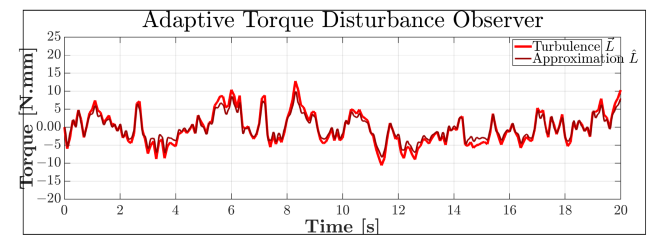
\includegraphics[width=\textwidth]{graphs/disturbance_L}
\vspace{-8pt}
\caption{Torque disturbance observer}
\label{fig:disturbance_L}
\end{subfigure}
\begin{subfigure}{\textwidth}
\centering
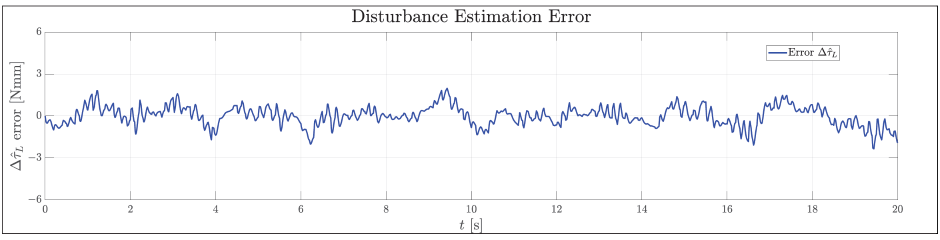
\includegraphics[width=\textwidth]{graphs/error_LR}
\vspace{-8pt}
\caption{Torque disturbance error deviation $\Delta\hat{\tau}_L$}
\label{fig:error_LR}
\end{subfigure}
\vspace{-6pt}
\caption{Adaptive disturbance observer example}
\label{fig:example_L}
\vspace{-12pt}
\end{figure}
%====================================================
\section{Position Control}
\label{sec:control.position}
%====================================================
Only two plant dependent position control laws are derived here as attitude control is the primary focus. The attitude control loop is stabilized independently from the position loop (Eq:\ref{eq:quaternion-states-angular} and Eq:\ref{eq:quaternion-states-acceleration}). Because the body's relative position is defined in the inertial frame (Eq:\ref{eq:quaternion-states-velocity}), but its translational velocity is defined in the body frame (Eq:\ref{eq:quaternion-states-acceleration}), the attitude plant needs to be stabilized before the position plant can be addressed. A simple Proportional-Derivative structure is presented first as the reference case. Thereafter, an ideal backstepping controller, which is extended to an adaptive control law is derived. Recalling the differential equation for translational acceleration from Eq:\ref{eq:quaternion-states-acceleration}:
\begin{equation}\label{eq:position-deriv}
\dot{\vec{v}}_b=m_b^{-1}\big(-\vec{\omega}_b\times m_b\vec{v}_b+m_b\vec{G}_b+\vec{F}_\mu(\hat{u})\big)~~~~~\in\mathcal{F}^b
\end{equation}
Recall that the Coriolis acceleration term $-\vec{\omega_b}\times m_b\vec{v}_b$ is what couples the position loop to the attitude plant and that $\vec{G}_b$ is the gravitational acceleration transformed to the body frame. Most texts assume that under standard operating conditions (App:\ref{app:equations.standard}), the angular velocity is small if not negligible $\vec{\omega}_b\approx\vec{0}$. It then follows that the coupled Coriolis term is assumed to be negligible when the angular velocity term is small, $\vec{\omega}_b\times m\vec{v}_b\approx \vec{0}$. 
\par
If the plant's state can be estimated with a relative degree of certainty, it is then easy to compensate for the coupled dynamics, rather than making assumptions about their influence on the system. In general, for the position control problem, translational velocity $\vec{v}_b$ is defined in the body frame and is related to the inertial position rates through a quaternion transformation:
\begin{equation}
\dot{\vec{\mathcal{E}}}_b=Q_b\otimes\vec{v}_b\otimes Q_b^*~~~~\in\mathcal{F}^I
\end{equation}
The difference in reference frames is an important distinction between the position and attitude state equations. Position error is calculated as the difference between a particular setpoint $\vec{\mathcal{E}}_d$ and the current body position $\vec{\mathcal{E}}_b$, which are both defined in the inertial frame:
\begin{equation}
\vec{\mathcal{E}}_e=\vec{\mathcal{E}}_d-\vec{\mathcal{E}}_b~~~~\in\mathcal{F}^I
\end{equation}
The translational position rate error $\dot{\vec{\mathcal{E}}}_b(t)$, \emph{not velocity error} $\vec{v}_e$, is calculated in the same way. Only first order setpoints are considered for the control laws presented here, so both position rate and velocity setpoints are zero, $\dot{\vec{\mathcal{E}}}_d=\vec{v}_d=\vec{0}$. The translational velocity error is then calculated as follows:
\begin{subequations}
\begin{equation}\label{eq:4.85a}
\dot{\vec{\mathcal{E}}}_e=\dot{\vec{\mathcal{E}}}_d-\dot{\vec{\mathcal{E}}}_b=-\dot{\vec{\mathcal{E}}}_b\Big|_{\dot{\vec{\mathcal{E}}}_d=\vec{0}}~~~~\in\mathcal{F}^{I}
\end{equation}
\vspace{-8pt}
\begin{equation}
\therefore \vec{v}_e = Q_b^*\otimes\big(\dot{\vec{\mathcal{E}}}_d-\dot{\vec{\mathcal{E}}}_b\big)\otimes Q_b = -\vec{v}_b~~~~\in\mathcal{F}^{b}
\end{equation}
\end{subequations}
Position setpoint tracking aims is to produce a stabilizing control law $g(\vec{\mathbf{x}}_e,\dot{\vec{\mathbf{x}}}_e,t)$ that ensures the position tracking error asymptotically tends to $\vec{0}$. Or more formally that:
\begin{subequations}
\begin{equation}
\vec{F}_\mu(\hat{u})=g\Big(\vec{\mathcal{E}}_d,\vec{v}_d,\vec{\mathcal{E}}_b,\vec{v}_b,t\Big)\equiv g(\vec{\mathcal{E}}_e,\dot{\vec{\mathcal{E}}}_e,t)~~~~\in\mathcal{F}^b
\end{equation}
\vspace{-18pt}
\begin{equation}
\text{such that:}~~\underset{t\rightarrow\infty}{\lim}\vec{\mathcal{E}}_e\rightarrow\vec{0}
\end{equation}
\end{subequations}
%====================================================
\subsection{PD Controller}
\label{subsec:control.position.pd}
%==================================================== 
Starting with a simple PD controller to be used for the reference case, plant dependent control designs the net force proportional to both the position error and the first derivative velocity error and compensates for plant dynamics:
\begin{subequations}\label{eq:position-pd}
\begin{equation}
\vec{F}_{_{PD}}=K_p\vec{\mathcal{E}}_e+K_d\dot{\vec{\mathcal{E}}}_e+\hat{\omega}_b\times m_b\hat{v}_b-m_b\vec{G}_b~~~~\in\mathcal{F}^b
\end{equation}
\vspace{-16pt}
\begin{equation}
=K_p\big(\vec{\mathcal{E}}_d-\hat{\mathcal{E}}_b\big)-K_d\big(\dot{\hat{\mathcal{E}}}_b\big)+\hat{\omega}_b\times m_b\hat{v}_b-m_b\vec{G}_b\Big|_{\dot{\vec{\mathcal{E}}}_e=-\dot{\hat{\mathcal{E}}}_b}
\end{equation}
\end{subequations}
where $K_p$ and $K_d$ are both $[3\times 3]$ symmetric positive definite gain coefficient matrices. Note that position and attitude state estimates are used for the controller in Eq:\ref{eq:position-pd}. As with attitude state estimates, it is assumed those estimates are error free and any plant errors are incorporated into the subsequent adaptive control law presented next in Sec:\ref{subsec:control.position.bacstepping}. The stability proof requires that error states are transformed to the body frame $\mathcal{F}^b$ from their principle inertial frame $\mathcal{F}^I$ such that the control input and error states act in a shared frame. Defining a position error state $\vec{X}_e$ that is transformed to the body frame:
\begin{subequations}
\begin{equation}\label{eq:4.80a}
\vec{X}_e\triangleq Q_b\otimes(\vec{\mathcal{E}}_d-\vec{\mathcal{E}}_b)\otimes Q_b^*=\vec{X}_d-\vec{X}_b~~~~\in\mathcal{F}^{b}
\end{equation}
Reiterating the difference between position rates and translational velocity in Eq:\ref{eq:quaternion-states-velocity}, position rates:
\begin{equation}\label{eq:4.80b}
\dot{\vec{X}}_e\triangleq Q_b\otimes(\dot{\vec{\mathcal{E}}}_d-\dot{\vec{\mathcal{E}}}_b)\otimes Q_b^*=-Q_b\otimes\dot{\vec{\mathcal{E}}}_b\otimes Q_b^* = -\vec{v}_b\Big|_{\dot{\vec{\mathcal{E}}}_d=\vec{0}}
\end{equation}
\end{subequations}
\emph{\color{gray}Quaternion derivatives for $\dot{Q}_b$ are not considered in Eq:\ref{eq:4.80b}. Only first order attitude setpoints were applied in Sec:\ref{subsec:control.attitude.controllers} so it is assumed quaternion rates will not affect the instantaneous transformation of translational position states. If the attitude control loop tracked non-zero angular velocities in Eq:\ref{eq:4.27c} then this would not be the case.}
\\
The control law from Eq:\ref{eq:position-pd}, despite being $\in\mathcal{F}^b$ has arguments $\vec{\mathcal{E}}_e,\dot{\vec{\mathcal{E}}}_e\in\mathcal{F}^I$, which are substituted with the transformed position error $\vec{X}_e$ and its rate $\dot{\vec{X}}_e$:
\begin{subequations}
\begin{equation}
\vec{F}_{_{PD}}=K_p\vec{X}_e + K_d\dot{\vec{X}}_e + \hat{\omega}_b\times m_b\hat{v}_b-m_b\vec{G}_b~~~~\in\mathcal{F}^{b}
\end{equation}
\vspace{-18pt}
\begin{equation}
=K_p\vec{X}_e-K_d\hat{v}_b+\hat{\omega}_b\times m_b\hat{v}_b-m_b\vec{G}_b
\end{equation}
\end{subequations}
Then proposing a positive definite Lyapunov function candidate:
\begin{subequations}
\begin{equation}
V_{_{PD}}(\vec{X}_e,\vec{v}_e)=\frac{1}{2}\vec{X}_e\text{}^TK_p\vec{X}_e+\frac{1}{2}\vec{v}_e\text{}^Tm_b\vec{v}_e>0~~~\forall(\vec{X}_e,\vec{v}_e)\not = \vec{0}
\end{equation}
\vspace{-12pt}
\begin{equation}
=\frac{1}{2}\vec{X}_e\text{}^TK_p\vec{X}_e+\frac{1}{2}\vec{v}_b\text{}^Tm_b\vec{v}_b\Big|_{\vec{v}_e=-\vec{v}_b}
\end{equation}
\end{subequations}
Calculating that LFC's derivative $\dot{V}_{_{PD}}$ with the PD control law substituted:
\begin{subequations}
\begin{equation}
\dot{V}_{_{PD}}(\vec{X}_e,\vec{v}_e)=\vec{X}_e\text{}^TK_p\dot{\vec{X}}_e+\vec{v}_b\text{}^Tm_b\dot{\vec{v}}_b
\end{equation}
\vspace{-10pt}
\begin{equation}
=-\vec{X}_e\text{}^TK_p\vec{v}_b+\vec{v}_b\text{}^Tm_b\dot{\vec{v}}_b
\end{equation}
\vspace{-8pt}
\begin{equation}
=-\vec{X}_e\text{}^TK_p\vec{v}_b+\vec{v}_b\text{}^T\big(-\vec{\omega}_b\times m_b\vec{v}_b+m_b\vec{G}_b+\vec{F}_{_{PD}}\big)
\end{equation}
\vspace{-8pt}
\begin{equation}
=-\vec{X}_e\text{}^TK_p \vec{v}_b+\vec{v}_b\text{}^T\big(K_p \vec{X}_e-K_d\hat{v}_b\big)
\end{equation}
\vspace{-8pt}
\begin{equation}\label{eq:position-pd-stability}
\therefore\dot{V}_{_{PD}}=-\vec{v}_b\text{}^TK_d\vec{v}_b~~<0,~\forall(\vec{X}_e,\vec{v}_e),~\exists(K_d,K_p)>0
\end{equation}
\end{subequations}
The global stability asserted in Eq:\ref{eq:position-pd-stability} holds $\forall(\vec{\mathcal{E}}_e,\dot{\vec{\mathcal{E}}}_e)$, irrespective of the transformation applied in Eq:\ref{eq:4.80a} and Eq:\ref{eq:4.80b}. The global asymptotically stabilizing limits then follow:
\begin{subequations}
\begin{equation}
\underset{t\rightarrow\infty}{\lim}\vec{X}_e=Q_b\otimes(\vec{\mathcal{E}}_d-\vec{\mathcal{E}}_b)\otimes Q_b^*\rightarrow\vec{0}
\end{equation}
\vspace{-10pt}
\begin{equation}
\therefore\underset{t\rightarrow\infty}{\lim}\vec{\mathcal{E}}_b\rightarrow\vec{\mathcal{E}}_d
\end{equation}
\vspace{-6pt}
\begin{equation}
\underset{t\rightarrow\infty}{\lim}\dot{X}_e=Q_b^*\otimes(\dot{\vec{\mathcal{E}}}_d-\dot{\vec{\mathcal{E}}}_b)\otimes Q_b=-\vec{v}_b\rightarrow\vec{0}\Big|_{\dot{\vec{\mathcal{E}}}_e=0}
\end{equation}
\end{subequations}
%====================================================
\subsection{Adaptive Backstepping Controller}
\label{subsec:control.position.bacstepping}
%====================================================
An adaptive backstepping algorithm, analogue to the adaptive controller previously in Sec:\ref{subsubsec:control.attitude.nonlinear.adaptivebackstep}, is now applied to position control. The disturbance force term $\vec{F}_D\in\mathcal{F}^b$ represents estimate errors together with any unmodelled lumped drag \emph{and} wind forces encountered by the vehicle in flight. That force disturbance is introduced to the position state differential Eq:\ref{eq:position-deriv}. Backstepping iterations for the position control loop first need to stabilize the position error, and only thereafter compensate for those disturbances (solving for an ideal backstepping controller first then adding adaptivity).
\begin{equation}\label{eq:4.99}
\dot{\vec{v}}_b=m_b^{-1}\big(-\vec{\omega}_b\times m_b\vec{v}_b+m_b\vec{G}_b+\vec{F}_D+\vec{F}_{_{ABC}}\big)~~~~\in\mathcal{F}^b
\end{equation}
The compensation for $\vec{F}_D$ is obviously an approximation for that physical disturbance term $\hat{F}_D$, beginning the backstepping process for position with a position state tracking error:
\begin{equation}
\vec{z}_1\triangleq\vec{\mathcal{E}}_d-\vec{\mathcal{E}}_b=\vec{\mathcal{E}}_e~~~~\in\mathcal{F}^{I}
\end{equation}
That backstepping error has its own derivative:
\begin{subequations}
\begin{equation}
\dot{\vec{z}}_1=\dot{\vec{\mathcal{E}}}_e=\dot{\vec{\mathcal{E}}}_d-\dot{\vec{\mathcal{E}}}_b
\end{equation}
\vspace{-12pt}
\begin{equation}
=Q_b^*\otimes \big(\vec{v}_d-\vec{v}_b\big)\otimes Q_b 
\end{equation}
\vspace{-12pt}
\begin{equation}
= - Q_b^*\otimes \vec{v}_b\otimes Q_b\Big|_{\vec{v}_d=\vec{0}}
\end{equation}
\end{subequations}
Transforming that error $\vec{z}_1$ to the body frame $\mathcal{F}^b$, in a similar fashion to Eq:\ref{eq:4.80a}, makes the stability proof more concise. The reference frame transformation does not affect the Layupanov candidate function's derivative as the energy function's gradient depends on its partial derivative with respect to its position trajectory only, namely $\mathcal{E}_e(t)$.
\begin{subequations}
\begin{equation}\label{eq:102a}
\vec{\zeta}_1\triangleq Q_b\otimes \vec{z}_1 \otimes Q_b^* =Q_b\otimes\big(\vec{\mathcal{E}}_d-\vec{\mathcal{E}}_b\big)\otimes Q_b^*=\vec{X}_e~~~~\in\mathcal{F}^{b}
\end{equation}
\vspace{-10pt}
\begin{equation}
\therefore \dot{\vec{\zeta}}_1=Q_b\otimes\dot{\vec{z}}_1\otimes Q_b^* = Q_b\otimes\big(\dot{\vec{\mathcal{E}}}_d-\dot{\vec{\mathcal{E}}}_b\big)\otimes Q_b^* = -\vec{v}_b
\end{equation}
\end{subequations}
Proposing the first Lyapunov function candidate $V_1(\vec{\zeta}_1)$ in terms of the tracking error:
\begin{subequations}
\begin{equation}\label{eq:103.a}
V_1(\vec{\zeta}_1)=\frac{1}{2}\vec{\zeta}_1\text{}^{T}\vec{\zeta}_1>0~~\forall(\vec{\zeta}_1)\not = \vec{0}
\end{equation}
which has a derivative:
\begin{equation}\label{eq:position-lyapunov-derivative}
\dot{V}_1(\vec{\zeta}_1)=\vec{\zeta}_1\text{}^T\dot{\vec{\zeta}}_1=-\vec{\zeta}_1\text{}^T\vec{v}_b
\end{equation}
\end{subequations}
The first backstepping control velocity in $\vec{\gamma}_d$ is the commanded input velocity for $\vec{v}_b$. Choosing $\vec{\gamma}_d$, so that when it is substituted for $\vec{v}_b$ the LFC derivative Eq:\ref{eq:position-lyapunov-derivative} is negative definite:
\begin{subequations}
\begin{equation}
\gamma_d \triangleq \Gamma_1 \vec{\zeta}_1
\end{equation}
where $\Gamma_1$ is a symmetric positive definite $[3\times 3]$ gain coefficient matrix. That commanded backstepping input has an error between the desired $\vec{\gamma}_d$ and the angular translational velocity $\vec{v}_b$. The error is the second backstepping error $\vec{\zeta}_2$ and is defined:
\begin{equation}
\vec{\zeta}_2 \triangleq \vec{\gamma}_d - \vec{v}_b = \Gamma_1\vec{\zeta}_1-\vec{v}_b
\end{equation}
\vspace{-15pt}
\begin{equation}\label{eq:4.90c}
\therefore \vec{v}_b=\Gamma_1\vec{\zeta}_1-\vec{\zeta}_2
\end{equation}
\end{subequations}
Substituting Eq:\ref{eq:4.90c} into the Lyapunov candidate function derivative $\dot{V}_1$ from Eq:\ref{eq:position-lyapunov-derivative} gives:
\begin{equation}\label{eq:105}
\dot{V}_1=-\vec{\zeta}_1\text{}^T\vec{v}_b=-\vec{\zeta}_1\text{}^T\Gamma_1\vec{\zeta}_1+\vec{\zeta}_1\text{}^T\vec{\zeta}_2
\end{equation}
The second backstepping error state $\vec{\zeta}_2$ has a derivative:
\begin{subequations}
\begin{equation}
\dot{\vec{\zeta}}_2=\dot{\vec{\gamma}}_d-\dot{\vec{v}}_b=\Gamma_1\dot{\vec{\zeta}}_1-\dot{\vec{v}}_b
\end{equation}
Introducing the translational acceleration differential equation for $\dot{\vec{v}}_b$ from Eq:\ref{eq:4.99}:
\begin{equation}\label{eq:102b}
\therefore\dot{\vec{\zeta}}_2=-\Gamma_1\vec{v}_b-m_b^{-1}\big(-\vec{\omega}_b\times m_b\vec{v}_b+m_b\vec{G}_b+\vec{F}_D+\vec{F}_{_{ABC}}\big)
\end{equation}
\end{subequations}
In order to stabilize the second backstepping error $\vec{\zeta}_2$, it is added as a trajectory variable to a new positive definite Lyapunov function candidate $V_2$ which extends from the first $V_1$ in Eq:\ref{eq:103.a}:
\begin{subequations}\label{eq:4.107a}
\begin{equation}
V_2(\vec{\zeta}_1,\vec{\zeta}_2)=V_1(\vec{\zeta}_1)+\frac{1}{2}\vec{\zeta}_2\text{}^T\vec{\zeta}_2
\end{equation}
\vspace{-12pt}
\begin{equation}
=\frac{1}{2}\vec{\zeta}_1\text{}^T\vec{\zeta}_1+\frac{1}{2}\vec{\zeta}_2\text{}^T\vec{\zeta}_2>0~~\forall(\hat{\zeta}_1,\vec{\zeta}_2)\not=\vec{0}
\end{equation}
\end{subequations}
That second Lyapunov function candidate has a derivative $\dot{V}_2$:
\begin{subequations}
\begin{equation}
\dot{V}_2(\vec{\zeta}_1,\vec{\zeta}_2)=\dot{V}_1(\vec{\zeta}_1)+\vec{\zeta}_2\text{}^T\dot{\vec{\zeta}}_2=\vec{\zeta}_1\text{}^T\dot{\vec{\zeta}}_1+\vec{\zeta}_2\text{}^T\dot{\vec{\zeta}}_2
\end{equation}
Inserting the first LFC derivative $\dot{V}_1$ from Eq:\ref{eq:105}:
\begin{equation}
\therefore\dot{V}_2=-\vec{\zeta}_1^T\Gamma_1\vec{\zeta}_1+\vec{\zeta}_1\text{}^T\vec{\zeta}_2+\vec{\zeta}_2\text{}^T\dot{\vec{\zeta}}_2
\end{equation}
Substituting the backstepping error's derivative $\dot{\vec{\zeta}}_2$ from Eq:\ref{eq:102b} gives:
\begin{equation}
\dot{V}_2=-\vec{\zeta}_1\text{}^T\Gamma_1\vec{\zeta}_1+\vec{\zeta}_2\text{}^T\bigg(\vec{\zeta
}_1-\Gamma_1\vec{v}_b-m_b^{-1}\big(-\vec{\omega}_b\times m_b\vec{v}_b+m\vec{G}_b+\vec{F}_D+\vec{F}_{_{IBC}}\big)\bigg)
\end{equation}
\end{subequations}
An ideal backstepping control law, assuming that $\vec{F}_D$ is known without errors, is then:
\begin{subequations}
\begin{equation}
\vec{F}_{_{IBC}}=m_b\big(\vec{\zeta}_1-\Gamma_1\hat{v}_b+\Gamma_2\vec{\zeta}_2\big)+\hat{\omega}_b\times m_b\hat{v}_b-m_b\vec{G}_b-\vec{F}_D~~~~\in\mathcal{F}^{b}
\end{equation}
\vspace{-12pt}
\begin{equation}
=m_b\Big(\big(1+\Gamma_1\Gamma_2\big)\vec{\zeta}_1-\big(\Gamma_1+\Gamma_2\big)\hat{v}_b\big)\Big)+\hat{\omega}_b\times m_b\hat{v}_b-m_b\vec{G}_b-\vec{F}_D
\end{equation}
where $\Gamma_2$ is another symmetric positive definite $[3\times 3]$ coefficient gain matrix. When that backstepping control law is substituted back into $\dot{V}_2$, the LFC derivative becomes negative definite:
\begin{equation}\label{eq:4.109c}
\therefore\dot{V}_{_{IBC}}=\dot{V}_2=-\vec{\zeta}_1\text{}^T\Gamma_1\vec{\zeta}_1-\vec{\zeta}_2\text{}^T\Gamma_2\vec{\zeta}_2<0~~\forall(\vec{\zeta}_1,\vec{\zeta}_2),~\exists(\Gamma_1,\Gamma_2)>0
\end{equation}
\end{subequations}
which leads to global asymptotic stability, assuming that the disturbance term $\vec{F}_D$ is known and can be compensated for without error. In the controller, both $\Gamma_1$ and $\Gamma_2$ are positive symmetric control coefficient matrices to be optimized. 
\par
The ideal backstepping rule and its associated Lyapunov function are now extended to incorporate an adaptive disturbance observer $\hat{F}_D$, similar to the adaptive backstepping attitude controller in Sec:\ref{subsubsec:control.attitude.nonlinear.adaptivebackstep}. The approximation leads to an estimate error $\Delta\hat{F}_D$:
\begin{subequations}
\begin{equation}
\Delta\hat{F}_D=\vec{F}_D-\hat{F}_b~~~~\in\mathcal{F}^b
\end{equation}
If it is assumed that the physical disturbance rates $\dot{\vec{F}}_D$ are far slower than the control dynamics, then $\dot{\vec{F}}_D<<\dot{\hat{F}}_D$:
\begin{equation}\label{eq:4.110b}
\Delta\dot{\vec{F}}_D=\dot{\vec{F}}_D-\dot{\hat{F}}_D\approx\vec{0}-\dot{\hat{F}}_D=-\dot{\hat{F}}_D\Big|_{\dot{\vec{F}}_D\approx\vec{0}}
\end{equation}
The adaptive control law then generates a force input that compensates for the phsyical disturbance $\vec{F}_D$ using the disturbance estimate $\hat{F}_D$:
\begin{equation}
\vec{F}_{_{ABC}}=m_b\big(\vec{\zeta}_1-\Gamma_1\hat{v}_b+\Gamma_2\vec{\zeta}_2\big)+\hat{\omega}_b\times m_b\hat{v}_b-m_b\vec{G}_b-\hat{F}_D~~~~\in\mathcal{F}^b
\end{equation}
\end{subequations}
Proposing a Lyapunov function candidate which extends from the ideal backstepping case in Eq:\ref{eq:4.107a} to include the disturbance estimate error $\Delta\hat{F}_D$ gives:
\begin{subequations}
\begin{equation}
V_{_{ABC}}(\vec{\zeta}_1,\vec{\zeta}_2,\Delta\hat{F}_D)= V_{_{IBC}}(\vec{\zeta}_1,\vec{\zeta}_2)+\frac{1}{2}\Delta\hat{F}_D\text{}^T\Gamma_D^{-1}\Delta\hat{F}_D
\end{equation}
where $\Gamma_D$ (much like $\Gamma_L$ in the adaptive attitude controller from Sec:\ref{subsec:control.attitude.nonlinear}) is a symmetric positive $[3\times 3]$ gain coefficient matrix which changes the response speed of the adaption plant. Then expanding the adaptive backstepping LFC $V_{_{ABC}}$ to prove it is positive definite:
\begin{equation}
V_{_{ABC}}=\frac{1}{2}\vec{\zeta}_1\text{}^T\vec{\zeta}_1+\frac{1}{2}\vec{\zeta}_2\text{}^T\vec{\zeta}_2+\frac{1}{2}\Delta\hat{F}_D\text{}^T\Gamma_D^{-1}\Delta\hat{F}_D>0~~\forall(\vec{\zeta}_1,\vec{\zeta}_2,\Delta\hat{F}_D)\not = \vec{0}
\end{equation}
Finding the LFC's derivative $\dot{V}_{_{ABC}}$ gives:
\begin{equation}
\dot{V}_{_{ABC}}=\vec{\zeta}_1\text{}^T\dot{\vec{\zeta}}_1+\vec{\zeta}_2\text{}^T\dot{\vec{\zeta}}_2+\Delta\hat{F}_D\text{}^T\Gamma_D^{-1}\Delta\dot{\hat{F}}_D
\end{equation}
and substituting derivatives for $\dot{\vec{\zeta}}_2$ from Eq:\ref{eq:102b} and $\Delta\dot{\hat{F}}_D$ from Eq:\ref{eq:4.110b}:
\begin{equation}
\dot{V}_{_{ABC}}=-\vec{\zeta}_1\text{}^T\Gamma_1\vec{\zeta}_1+\vec{\zeta}_2\text{}^T\bigg(\vec{\zeta}_1-\Gamma_1\vec{v}_b-m_b^{-1}\big(-\vec{\omega}_b\times m_b\vec{v}_b+m_b\vec{G}_b+\vec{F}_D+\vec{F}_{_{ABC}}\big)\bigg)-\vec{D}_\Delta^{~T}\Gamma_D^{-1}\dot{\hat{D}}
\end{equation}
Then expanding the adaptive backstepping controller generated force $\vec{F}_{_{ABC}}$:
\begin{equation}
\dot{V}_{_{ABC}}=-\vec{\zeta}_1\text{}^T\Gamma_1\vec{\zeta}_1+\vec{\zeta}_2\text{}^T\bigg(-\Gamma_2\vec{\zeta}_2-m_b^{-1}\big(\vec{F}_D-\hat{F}_D\big)\bigg)-\Delta\hat{F}_D\text{}^T\Gamma_D^{-1}\Delta\dot{\hat{F}}_D
\end{equation}
\vspace{-8pt}
\begin{equation}
=-\vec{\zeta}_1\text{}^T\Gamma_1\vec{\zeta}_1-\vec{\zeta}_2\text{}^T\Gamma_2\vec{\zeta}_2-m_b^{-1}\vec{\zeta}_2\text{}^T\Delta\hat{F}_D-\Delta\hat{F}_D\text{}^T\Gamma_D^{-1}\Delta\dot{\hat{F}}_D
\end{equation}
\vspace{-8pt}
\begin{equation}\label{eq:4.105g}
=-\vec{\zeta}_1\text{}^T\Gamma_1\vec{\zeta}_1-\vec{\zeta}_2\text{}^T\Gamma_2\vec{\zeta}_2-m_b^{-1}\Delta\hat{F}_D\text{}^T\Gamma_D^{-1}\big(\Gamma_D\vec{\zeta}_2+\Delta\dot{\hat{F}}_D\big)
\end{equation}
\end{subequations}
Then, a self-evident choice for the disturbance update law would be $\Delta\dot{\hat{F}}_D=-m^{-1}\Gamma_D\vec{\zeta}_2$, which ensures asymptotic stability:
\begin{subequations}
\begin{equation}\label{eq:abc-asymptotic-position}
\Delta\dot{\hat{F}}_D\triangleq-m_b^{-1}\Gamma_D\vec{\zeta}_2=-m_b^{-1}\Gamma_D\Big(\Gamma_1\vec{\zeta}_1-\vec{v}_b\Big)
\end{equation}
Substituting that into the LFC derivative Eq:\ref{eq:4.105g} produces:
\begin{equation}
\dot{V}_{_{ABC}}=-\vec{\zeta}_1\text{}^T\Gamma_1\vec{\zeta}_1-\vec{\zeta}_2\text{}^T\Gamma_2\vec{\zeta}_2<0~~\forall(\hat{z}_1,\hat{z}_2,\vec{D}_\Delta),~~\exists(\Gamma_1,\Gamma_2,\Gamma_\Delta)>0
\end{equation}
\end{subequations}
The disturbance observer tracks a general single axis directional force disturbance as illustrated in Fig:\ref{fig:disturbance_D}. That disturbance is a combined fluctuating wind force and vector field, the model of which is later described in Sec:\ref{subsec:simulation.disturbance.force}. Note that Fig:\ref{fig:example_D} tracks an \emph{open loop} disturbance on a vehicle stabilized steady state. An estimation error for the deviation from the physical disturbance is plotted in Fig:\ref{fig:error_DR}. 
\par
Again there is a damping between the physical and approximated forces, no new state information is used to estimate signals in both Fig:\ref{fig:disturbance_L} and Fig:\ref{fig:disturbance_D} for attitude and position disturbances respectively. Adaptive observers in Eq:\ref{eq:abc-asymptotic} and Eq:\ref{eq:abc-asymptotic-position} simply introduce additional free parameters to the control loop.
\begin{figure}[htbp]
\centering
\begin{subfigure}{\textwidth}
\centering
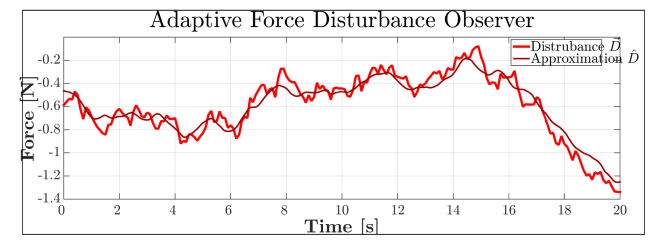
\includegraphics[width=\textwidth]{graphs/disturbance_D}
\vspace{-4pt}
\caption{Force disturbance observer}
\label{fig:disturbance_D}
\end{subfigure}
\begin{subfigure}{\textwidth}
\centering
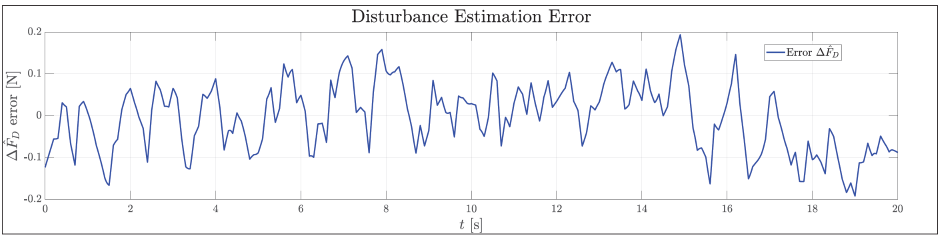
\includegraphics[width=\textwidth]{graphs/error_DR}
\vspace{-4pt}
\caption{Force disturbance error deviation $\Delta\hat{F}_D$}
\label{fig:error_DR}
\end{subfigure}
\vspace{-6pt}
\caption{Adaptive disturbance observer example}
\label{fig:example_D}
\end{figure}
